\documentclass[a4paper]{article}
\nonstopmode

\usepackage{listings}
\usepackage[T1]{fontenc}
\usepackage{color}
\usepackage{pxfonts}
\usepackage{pdfpages}

\definecolor{dkgreen}{rgb}{0,0.6,0}
\definecolor{gray}{rgb}{0.5,0.5,0.5}
\definecolor{mauve}{rgb}{0.58,0,0.82}


\lstset{frame=tb,
    aboveskip=3mm,
    belowskip=3mm,
    showstringspaces=false,
    columns=flexible,
    basicstyle={\small\ttfamily},
    numbers=none,
    numberstyle=\tiny\color{gray},
    keywordstyle=\color{blue},
    commentstyle=\color{dkgreen},
    stringstyle=\color{mauve},
    breaklines=true,
    breakatwhitespace=true,
    tabsize=3
}

\title{Gossip-based dissemination, Peer Sampling Service}

\author{Markus Roth}

\begin{document}

\maketitle

\tableofcontents

\section{Solution Overview}

\subsection{Introduction}

I created a single program that can be configured using constants at the top of the file. By changing these constants, it is possible to run all of the experiments in the assignment with the same piece of code. For each task, I have reproduced the configuration constants section of the program at the appropriate chapter in this document. To run the experiment, one needs to copy the configuration section into the correct section in gossip.lua and run it on the cluster. This section is marked with START CONFIG SECTION and END CONFIG SECTION.
I chose this approach to reduce code duplication and guarantee a consistent reproducability of all results presented.

\subsection{gossip.lua}

This is the program that runs the experiements. If follows the provided skeleton. It contains the implementation of the peer samplingn service as well as the implementation of the rumor mongering and anti-entropy protocols.

\subsection{parselog.lua}

This LUA-script reads a log file created by running an experiment and aggragates the log entries to be able to parse them. It reads from the file named in its first parameter and writes to the same filename with a prefix of aggregated\textunderscore . The aggregated log file contains the following columns:

\begin{enumerate}
\item relative\textunderscore time: The number of seconds passed from the start of the experiment
\item cycles: The number of cycles passed frmo the start of the experiment
\item absolute\textunderscore infected\textunderscore nodes: The absolute number of nodes that are infected
\item relative\textunderscore infected\textunderscore nodes: The relative number of nodes that are infected
\item nodes\textunderscore infected\textunderscore by\textunderscore anti\textunderscore entropy: The cumulative number of nodes infected by the anti-entropy prodocol.
\item nodes\textunderscore infected\textunderscore by\textunderscore rumor\textunderscore mongering: The cumulative number of nodes infected by the rumor mongering prodocol.
\end{enumerate}

\subsection{parselog.lua}

The same as parselog.lua, but sorts the entries by their relative time values rather than their cycles. Used for the second-plots.

\subsection{/plots}

These gnuplot scripts read from aggregated log files produced by parselog.lua. They produces a .tex files of the graphs in the /plots directory. These .tex files are then embedded in this report via latex includes.

There are many adaptions of the script used for this report. For each exercise, the script exists named after the exercise number and the parameters used.

Note that I plotted the graphs with cycles in the x axis. This is because we were asked to do so in the lab session. Since I think plots with seconds are more legible, I added them at some places as well.

The resulting .tex files are also included in the submission.

\section{Task 2.1.1}

Running gossip.lua with this configuration does what is required:

\begin{lstlisting}
---START CONFIG SECTION---
do_anti_entropy = true
gossip_interval = 5
max_cycles = 10
--END CONFIG SECTION---
\end{lstlisting}

\section{Task 2.1.2}

Running the code from section 2.1.1 on 40 peers on the splay cluster gives the following log:
\begin{lstlisting}
2016-10-24 13:55:02.972688 (92)     0 i_am_infected_as_patient_zero
2016-10-24 13:55:07.981443 (19)     0 i_am_infected_by_anti_entropy
2016-10-24 13:55:09.988781 (130)    1 i_am_infected_by_anti_entropy
2016-10-24 13:55:11.952454 (3)      1 i_am_infected_by_anti_entropy
2016-10-24 13:55:12.984608 (76)     1 i_am_infected_by_anti_entropy
2016-10-24 13:55:13.344219 (166)    2 i_am_infected_by_anti_entropy
2016-10-24 13:55:13.456906 (56)     1 i_am_infected_by_anti_entropy
2016-10-24 13:55:13.546528 (41)     2 i_am_infected_by_anti_entropy
2016-10-24 13:55:14.211685 (150)    2 i_am_infected_by_anti_entropy
2016-10-24 13:55:14.968156 (168)    2 i_am_infected_by_anti_entropy
2016-10-24 13:55:15.438669 (171)    2 i_am_infected_by_anti_entropy
2016-10-24 13:55:15.577630 (96)     2 i_am_infected_by_anti_entropy
2016-10-24 13:55:15.781953 (58)     2 i_am_infected_by_anti_entropy
2016-10-24 13:55:16.358811 (115)    2 i_am_infected_by_anti_entropy
2016-10-24 13:55:16.738897 (167)    2 i_am_infected_by_anti_entropy
2016-10-24 13:55:16.984977 (112)    2 i_am_infected_by_anti_entropy
2016-10-24 13:55:17.197953 (113)    2 i_am_infected_by_anti_entropy
2016-10-24 13:55:17.365741 (38)     3 i_am_infected_by_anti_entropy
2016-10-24 13:55:17.605150 (77)     3 i_am_infected_by_anti_entropy
2016-10-24 13:55:17.682568 (40)     3 i_am_infected_by_anti_entropy
2016-10-24 13:55:17.738057 (151)    3 i_am_infected_by_anti_entropy
2016-10-24 13:55:17.986358 (78)     2 i_am_infected_by_anti_entropy
2016-10-24 13:55:18.346416 (20)     2 i_am_infected_by_anti_entropy
2016-10-24 13:55:18.458532 (18)     2 i_am_infected_by_anti_entropy
2016-10-24 13:55:18.550194 (55)     2 i_am_infected_by_anti_entropy
2016-10-24 13:55:19.214494 (22)     2 i_am_infected_by_anti_entropy
2016-10-24 13:55:19.366339 (129)    3 i_am_infected_by_anti_entropy
2016-10-24 13:55:19.593522 (132)    3 i_am_infected_by_anti_entropy
2016-10-24 13:55:20.190240 (1)      3 i_am_infected_by_anti_entropy
2016-10-24 13:55:20.559921 (57)     3 i_am_infected_by_anti_entropy
2016-10-24 13:55:20.579709 (114)    3 i_am_infected_by_anti_entropy
2016-10-24 13:55:20.768034 (74)     3 i_am_infected_by_anti_entropy
2016-10-24 13:55:20.796862 (149)    3 i_am_infected_by_anti_entropy
2016-10-24 13:55:21.185359 (111)    3 i_am_infected_by_anti_entropy
2016-10-24 13:55:21.331993 (169)    3 i_am_infected_by_anti_entropy
2016-10-24 13:55:21.552212 (75)     3 i_am_infected_by_anti_entropy
2016-10-24 13:55:21.887625 (39)     3 i_am_infected_by_anti_entropy
2016-10-24 13:55:21.911745 (95)     3 i_am_infected_by_anti_gntropy
2016-10-24 13:55:22.369056 (133)    3 i_am_infected_by_anti_entropy
2016-10-24 13:55:25.245777 (148)    4 i_am_infected_by_anti_entropy
\end{lstlisting}

As we can see, dissemination is complete after around 4 cycles. Not included: Final messages by all nodes saying that they are indeed infected.

\section{Task 2.1.3}

The script for parsing logs can be found in the file parselog.lua.

\section{Task 2.1.4}

\begin{figure}
    % GNUPLOT: LaTeX picture with Postscript
\begingroup
  \makeatletter
  \providecommand\color[2][]{%
    \GenericError{(gnuplot) \space\space\space\@spaces}{%
      Package color not loaded in conjunction with
      terminal option `colourtext'%
    }{See the gnuplot documentation for explanation.%
    }{Either use 'blacktext' in gnuplot or load the package
      color.sty in LaTeX.}%
    \renewcommand\color[2][]{}%
  }%
  \providecommand\includegraphics[2][]{%
    \GenericError{(gnuplot) \space\space\space\@spaces}{%
      Package graphicx or graphics not loaded%
    }{See the gnuplot documentation for explanation.%
    }{The gnuplot epslatex terminal needs graphicx.sty or graphics.sty.}%
    \renewcommand\includegraphics[2][]{}%
  }%
  \providecommand\rotatebox[2]{#2}%
  \@ifundefined{ifGPcolor}{%
    \newif\ifGPcolor
    \GPcolorfalse
  }{}%
  \@ifundefined{ifGPblacktext}{%
    \newif\ifGPblacktext
    \GPblacktexttrue
  }{}%
  % define a \g@addto@macro without @ in the name:
  \let\gplgaddtomacro\g@addto@macro
  % define empty templates for all commands taking text:
  \gdef\gplbacktext{}%
  \gdef\gplfronttext{}%
  \makeatother
  \ifGPblacktext
    % no textcolor at all
    \def\colorrgb#1{}%
    \def\colorgray#1{}%
  \else
    % gray or color?
    \ifGPcolor
      \def\colorrgb#1{\color[rgb]{#1}}%
      \def\colorgray#1{\color[gray]{#1}}%
      \expandafter\def\csname LTw\endcsname{\color{white}}%
      \expandafter\def\csname LTb\endcsname{\color{black}}%
      \expandafter\def\csname LTa\endcsname{\color{black}}%
      \expandafter\def\csname LT0\endcsname{\color[rgb]{1,0,0}}%
      \expandafter\def\csname LT1\endcsname{\color[rgb]{0,1,0}}%
      \expandafter\def\csname LT2\endcsname{\color[rgb]{0,0,1}}%
      \expandafter\def\csname LT3\endcsname{\color[rgb]{1,0,1}}%
      \expandafter\def\csname LT4\endcsname{\color[rgb]{0,1,1}}%
      \expandafter\def\csname LT5\endcsname{\color[rgb]{1,1,0}}%
      \expandafter\def\csname LT6\endcsname{\color[rgb]{0,0,0}}%
      \expandafter\def\csname LT7\endcsname{\color[rgb]{1,0.3,0}}%
      \expandafter\def\csname LT8\endcsname{\color[rgb]{0.5,0.5,0.5}}%
    \else
      % gray
      \def\colorrgb#1{\color{black}}%
      \def\colorgray#1{\color[gray]{#1}}%
      \expandafter\def\csname LTw\endcsname{\color{white}}%
      \expandafter\def\csname LTb\endcsname{\color{black}}%
      \expandafter\def\csname LTa\endcsname{\color{black}}%
      \expandafter\def\csname LT0\endcsname{\color{black}}%
      \expandafter\def\csname LT1\endcsname{\color{black}}%
      \expandafter\def\csname LT2\endcsname{\color{black}}%
      \expandafter\def\csname LT3\endcsname{\color{black}}%
      \expandafter\def\csname LT4\endcsname{\color{black}}%
      \expandafter\def\csname LT5\endcsname{\color{black}}%
      \expandafter\def\csname LT6\endcsname{\color{black}}%
      \expandafter\def\csname LT7\endcsname{\color{black}}%
      \expandafter\def\csname LT8\endcsname{\color{black}}%
    \fi
  \fi
    \setlength{\unitlength}{0.0500bp}%
    \ifx\gptboxheight\undefined%
      \newlength{\gptboxheight}%
      \newlength{\gptboxwidth}%
      \newsavebox{\gptboxtext}%
    \fi%
    \setlength{\fboxrule}{0.5pt}%
    \setlength{\fboxsep}{1pt}%
\begin{picture}(7200.00,5040.00)%
    \gplgaddtomacro\gplbacktext{%
      \csname LTb\endcsname%
      \put(682,704){\makebox(0,0)[r]{\strut{}$0$}}%
      \csname LTb\endcsname%
      \put(682,1163){\makebox(0,0)[r]{\strut{}$5$}}%
      \csname LTb\endcsname%
      \put(682,1623){\makebox(0,0)[r]{\strut{}$10$}}%
      \csname LTb\endcsname%
      \put(682,2082){\makebox(0,0)[r]{\strut{}$15$}}%
      \csname LTb\endcsname%
      \put(682,2542){\makebox(0,0)[r]{\strut{}$20$}}%
      \csname LTb\endcsname%
      \put(682,3001){\makebox(0,0)[r]{\strut{}$25$}}%
      \csname LTb\endcsname%
      \put(682,3460){\makebox(0,0)[r]{\strut{}$30$}}%
      \csname LTb\endcsname%
      \put(682,3920){\makebox(0,0)[r]{\strut{}$35$}}%
      \csname LTb\endcsname%
      \put(682,4379){\makebox(0,0)[r]{\strut{}$40$}}%
      \csname LTb\endcsname%
      \put(814,484){\makebox(0,0){\strut{}$0$}}%
      \csname LTb\endcsname%
      \put(1563,484){\makebox(0,0){\strut{}$0.5$}}%
      \csname LTb\endcsname%
      \put(2311,484){\makebox(0,0){\strut{}$1$}}%
      \csname LTb\endcsname%
      \put(3060,484){\makebox(0,0){\strut{}$1.5$}}%
      \csname LTb\endcsname%
      \put(3809,484){\makebox(0,0){\strut{}$2$}}%
      \csname LTb\endcsname%
      \put(4557,484){\makebox(0,0){\strut{}$2.5$}}%
      \csname LTb\endcsname%
      \put(5306,484){\makebox(0,0){\strut{}$3$}}%
      \csname LTb\endcsname%
      \put(6054,484){\makebox(0,0){\strut{}$3.5$}}%
      \csname LTb\endcsname%
      \put(6803,484){\makebox(0,0){\strut{}$4$}}%
    }%
    \gplgaddtomacro\gplfronttext{%
      \csname LTb\endcsname%
      \put(176,2541){\rotatebox{-270}{\makebox(0,0){\strut{}Peers Infected}}}%
      \put(3808,154){\makebox(0,0){\strut{}Cycles}}%
      \put(3808,4709){\makebox(0,0){\strut{}Anti-Entropy Dissemination}}%
      \csname LTb\endcsname%
      \put(2794,4206){\makebox(0,0)[r]{\strut{}infected nodes}}%
    }%
    \gplbacktext
    \put(0,0){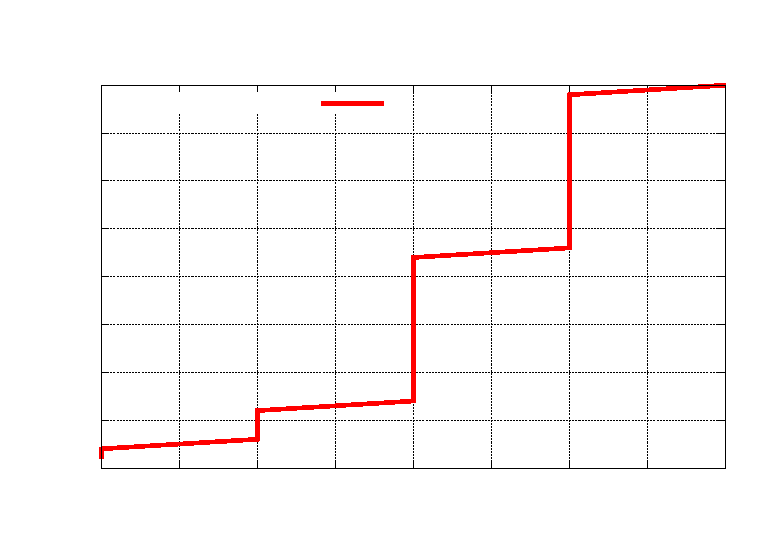
\includegraphics{plots/plot_2-1-4}}%
    \gplfronttext
  \end{picture}%
\endgroup

    \caption{Task 2.1.4: Anti-Entropy dissemination with 40 peers}
    \label{fig:2-1-4}
\end{figure}

The gnuplot script can be found in the file plot.gp. It might be modied in details to produce the various graphs in this report, but in general it remains the same.

Applying the script to the data gained in task 2.1.2, we get plot show in figure \ref{fig:2-1-4}.

\section{Task 2.2.1}
\begin{lstlisting}
---START CONFIG SECTION---
do_rumor_mongering = true
gossip_interval = 5
initial_hops_to_live = 3
distribution_count = 2
max_cycles = 5
---END CONFIG SECTION---
\end{lstlisting}


\begin{figure}
    % GNUPLOT: LaTeX picture with Postscript
\begingroup
  \makeatletter
  \providecommand\color[2][]{%
    \GenericError{(gnuplot) \space\space\space\@spaces}{%
      Package color not loaded in conjunction with
      terminal option `colourtext'%
    }{See the gnuplot documentation for explanation.%
    }{Either use 'blacktext' in gnuplot or load the package
      color.sty in LaTeX.}%
    \renewcommand\color[2][]{}%
  }%
  \providecommand\includegraphics[2][]{%
    \GenericError{(gnuplot) \space\space\space\@spaces}{%
      Package graphicx or graphics not loaded%
    }{See the gnuplot documentation for explanation.%
    }{The gnuplot epslatex terminal needs graphicx.sty or graphics.sty.}%
    \renewcommand\includegraphics[2][]{}%
  }%
  \providecommand\rotatebox[2]{#2}%
  \@ifundefined{ifGPcolor}{%
    \newif\ifGPcolor
    \GPcolorfalse
  }{}%
  \@ifundefined{ifGPblacktext}{%
    \newif\ifGPblacktext
    \GPblacktexttrue
  }{}%
  % define a \g@addto@macro without @ in the name:
  \let\gplgaddtomacro\g@addto@macro
  % define empty templates for all commands taking text:
  \gdef\gplbacktext{}%
  \gdef\gplfronttext{}%
  \makeatother
  \ifGPblacktext
    % no textcolor at all
    \def\colorrgb#1{}%
    \def\colorgray#1{}%
  \else
    % gray or color?
    \ifGPcolor
      \def\colorrgb#1{\color[rgb]{#1}}%
      \def\colorgray#1{\color[gray]{#1}}%
      \expandafter\def\csname LTw\endcsname{\color{white}}%
      \expandafter\def\csname LTb\endcsname{\color{black}}%
      \expandafter\def\csname LTa\endcsname{\color{black}}%
      \expandafter\def\csname LT0\endcsname{\color[rgb]{1,0,0}}%
      \expandafter\def\csname LT1\endcsname{\color[rgb]{0,1,0}}%
      \expandafter\def\csname LT2\endcsname{\color[rgb]{0,0,1}}%
      \expandafter\def\csname LT3\endcsname{\color[rgb]{1,0,1}}%
      \expandafter\def\csname LT4\endcsname{\color[rgb]{0,1,1}}%
      \expandafter\def\csname LT5\endcsname{\color[rgb]{1,1,0}}%
      \expandafter\def\csname LT6\endcsname{\color[rgb]{0,0,0}}%
      \expandafter\def\csname LT7\endcsname{\color[rgb]{1,0.3,0}}%
      \expandafter\def\csname LT8\endcsname{\color[rgb]{0.5,0.5,0.5}}%
    \else
      % gray
      \def\colorrgb#1{\color{black}}%
      \def\colorgray#1{\color[gray]{#1}}%
      \expandafter\def\csname LTw\endcsname{\color{white}}%
      \expandafter\def\csname LTb\endcsname{\color{black}}%
      \expandafter\def\csname LTa\endcsname{\color{black}}%
      \expandafter\def\csname LT0\endcsname{\color{black}}%
      \expandafter\def\csname LT1\endcsname{\color{black}}%
      \expandafter\def\csname LT2\endcsname{\color{black}}%
      \expandafter\def\csname LT3\endcsname{\color{black}}%
      \expandafter\def\csname LT4\endcsname{\color{black}}%
      \expandafter\def\csname LT5\endcsname{\color{black}}%
      \expandafter\def\csname LT6\endcsname{\color{black}}%
      \expandafter\def\csname LT7\endcsname{\color{black}}%
      \expandafter\def\csname LT8\endcsname{\color{black}}%
    \fi
  \fi
    \setlength{\unitlength}{0.0500bp}%
    \ifx\gptboxheight\undefined%
      \newlength{\gptboxheight}%
      \newlength{\gptboxwidth}%
      \newsavebox{\gptboxtext}%
    \fi%
    \setlength{\fboxrule}{0.5pt}%
    \setlength{\fboxsep}{1pt}%
\begin{picture}(7200.00,5040.00)%
    \gplgaddtomacro\gplbacktext{%
      \csname LTb\endcsname%
      \put(682,704){\makebox(0,0)[r]{\strut{}$0$}}%
      \csname LTb\endcsname%
      \put(682,1163){\makebox(0,0)[r]{\strut{}$5$}}%
      \csname LTb\endcsname%
      \put(682,1623){\makebox(0,0)[r]{\strut{}$10$}}%
      \csname LTb\endcsname%
      \put(682,2082){\makebox(0,0)[r]{\strut{}$15$}}%
      \csname LTb\endcsname%
      \put(682,2542){\makebox(0,0)[r]{\strut{}$20$}}%
      \csname LTb\endcsname%
      \put(682,3001){\makebox(0,0)[r]{\strut{}$25$}}%
      \csname LTb\endcsname%
      \put(682,3460){\makebox(0,0)[r]{\strut{}$30$}}%
      \csname LTb\endcsname%
      \put(682,3920){\makebox(0,0)[r]{\strut{}$35$}}%
      \csname LTb\endcsname%
      \put(682,4379){\makebox(0,0)[r]{\strut{}$40$}}%
      \csname LTb\endcsname%
      \put(814,484){\makebox(0,0){\strut{}$0$}}%
      \csname LTb\endcsname%
      \put(2311,484){\makebox(0,0){\strut{}$0.5$}}%
      \csname LTb\endcsname%
      \put(3809,484){\makebox(0,0){\strut{}$1$}}%
      \csname LTb\endcsname%
      \put(5306,484){\makebox(0,0){\strut{}$1.5$}}%
      \csname LTb\endcsname%
      \put(6803,484){\makebox(0,0){\strut{}$2$}}%
    }%
    \gplgaddtomacro\gplfronttext{%
      \csname LTb\endcsname%
      \put(176,2541){\rotatebox{-270}{\makebox(0,0){\strut{}Peers Infected}}}%
      \put(3808,154){\makebox(0,0){\strut{}Cycles}}%
      \put(3808,4709){\makebox(0,0){\strut{}Rumor Mongering Dissemination}}%
      \csname LTb\endcsname%
      \put(2794,4206){\makebox(0,0)[r]{\strut{}infected nodes}}%
    }%
    \gplbacktext
    \put(0,0){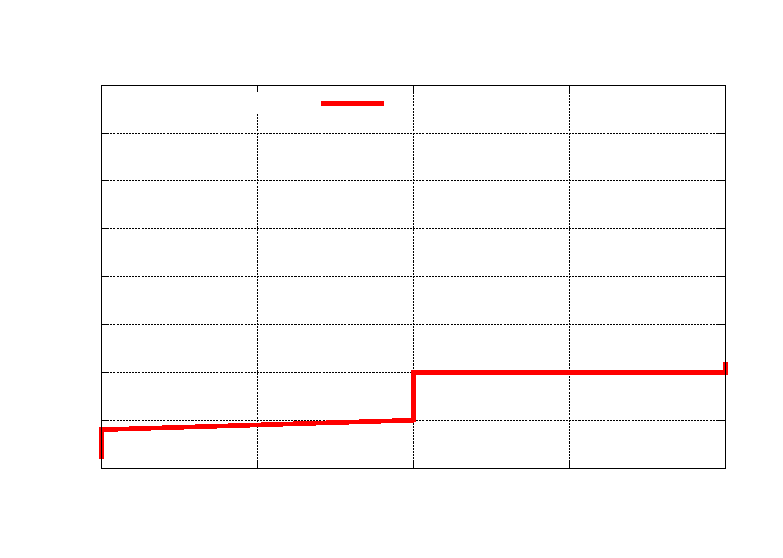
\includegraphics{plots/plot_2-2-1}}%
    \gplfronttext
  \end{picture}%
\endgroup

    \caption{Task 2.2.1: Rumor Mongering dissemination with 40 peers (HTL=3, f=2)}
    \label{fig:2-2-1}
\end{figure}

The results of the experiment can be found in \ref{fig:2-2-1}. As we can see, 12 nodes were infected and two duplicates received, leading to the expected number of 14 recipients of a rumor. Since the cycles are not aligned, calls tend to move from cycle n to cyle n-1, because cycle n-1 runs first. This is the reason we see all infection shappen within cycles 0 to 3, rather than the last infections only happening in cycle 3.


\section{Task 2.2.2}

The log of Task 2.2.1 lists the incoming messages by rumor mongering:

\lstinputlisting{logs/log_2-2-1.txt}

Again we note that the cycles are not aligned, so we see the infections happing in an earlier cycle than they have been issued.

\section{Task 2.2.3}

\begin{figure}
    % GNUPLOT: LaTeX picture with Postscript
\begingroup
  \makeatletter
  \providecommand\color[2][]{%
    \GenericError{(gnuplot) \space\space\space\@spaces}{%
      Package color not loaded in conjunction with
      terminal option `colourtext'%
    }{See the gnuplot documentation for explanation.%
    }{Either use 'blacktext' in gnuplot or load the package
      color.sty in LaTeX.}%
    \renewcommand\color[2][]{}%
  }%
  \providecommand\includegraphics[2][]{%
    \GenericError{(gnuplot) \space\space\space\@spaces}{%
      Package graphicx or graphics not loaded%
    }{See the gnuplot documentation for explanation.%
    }{The gnuplot epslatex terminal needs graphicx.sty or graphics.sty.}%
    \renewcommand\includegraphics[2][]{}%
  }%
  \providecommand\rotatebox[2]{#2}%
  \@ifundefined{ifGPcolor}{%
    \newif\ifGPcolor
    \GPcolorfalse
  }{}%
  \@ifundefined{ifGPblacktext}{%
    \newif\ifGPblacktext
    \GPblacktexttrue
  }{}%
  % define a \g@addto@macro without @ in the name:
  \let\gplgaddtomacro\g@addto@macro
  % define empty templates for all commands taking text:
  \gdef\gplbacktext{}%
  \gdef\gplfronttext{}%
  \makeatother
  \ifGPblacktext
    % no textcolor at all
    \def\colorrgb#1{}%
    \def\colorgray#1{}%
  \else
    % gray or color?
    \ifGPcolor
      \def\colorrgb#1{\color[rgb]{#1}}%
      \def\colorgray#1{\color[gray]{#1}}%
      \expandafter\def\csname LTw\endcsname{\color{white}}%
      \expandafter\def\csname LTb\endcsname{\color{black}}%
      \expandafter\def\csname LTa\endcsname{\color{black}}%
      \expandafter\def\csname LT0\endcsname{\color[rgb]{1,0,0}}%
      \expandafter\def\csname LT1\endcsname{\color[rgb]{0,1,0}}%
      \expandafter\def\csname LT2\endcsname{\color[rgb]{0,0,1}}%
      \expandafter\def\csname LT3\endcsname{\color[rgb]{1,0,1}}%
      \expandafter\def\csname LT4\endcsname{\color[rgb]{0,1,1}}%
      \expandafter\def\csname LT5\endcsname{\color[rgb]{1,1,0}}%
      \expandafter\def\csname LT6\endcsname{\color[rgb]{0,0,0}}%
      \expandafter\def\csname LT7\endcsname{\color[rgb]{1,0.3,0}}%
      \expandafter\def\csname LT8\endcsname{\color[rgb]{0.5,0.5,0.5}}%
    \else
      % gray
      \def\colorrgb#1{\color{black}}%
      \def\colorgray#1{\color[gray]{#1}}%
      \expandafter\def\csname LTw\endcsname{\color{white}}%
      \expandafter\def\csname LTb\endcsname{\color{black}}%
      \expandafter\def\csname LTa\endcsname{\color{black}}%
      \expandafter\def\csname LT0\endcsname{\color{black}}%
      \expandafter\def\csname LT1\endcsname{\color{black}}%
      \expandafter\def\csname LT2\endcsname{\color{black}}%
      \expandafter\def\csname LT3\endcsname{\color{black}}%
      \expandafter\def\csname LT4\endcsname{\color{black}}%
      \expandafter\def\csname LT5\endcsname{\color{black}}%
      \expandafter\def\csname LT6\endcsname{\color{black}}%
      \expandafter\def\csname LT7\endcsname{\color{black}}%
      \expandafter\def\csname LT8\endcsname{\color{black}}%
    \fi
  \fi
    \setlength{\unitlength}{0.0500bp}%
    \ifx\gptboxheight\undefined%
      \newlength{\gptboxheight}%
      \newlength{\gptboxwidth}%
      \newsavebox{\gptboxtext}%
    \fi%
    \setlength{\fboxrule}{0.5pt}%
    \setlength{\fboxsep}{1pt}%
\begin{picture}(7200.00,5040.00)%
    \gplgaddtomacro\gplbacktext{%
      \csname LTb\endcsname%
      \put(682,704){\makebox(0,0)[r]{\strut{}$0$}}%
      \csname LTb\endcsname%
      \put(682,1163){\makebox(0,0)[r]{\strut{}$5$}}%
      \csname LTb\endcsname%
      \put(682,1623){\makebox(0,0)[r]{\strut{}$10$}}%
      \csname LTb\endcsname%
      \put(682,2082){\makebox(0,0)[r]{\strut{}$15$}}%
      \csname LTb\endcsname%
      \put(682,2542){\makebox(0,0)[r]{\strut{}$20$}}%
      \csname LTb\endcsname%
      \put(682,3001){\makebox(0,0)[r]{\strut{}$25$}}%
      \csname LTb\endcsname%
      \put(682,3460){\makebox(0,0)[r]{\strut{}$30$}}%
      \csname LTb\endcsname%
      \put(682,3920){\makebox(0,0)[r]{\strut{}$35$}}%
      \csname LTb\endcsname%
      \put(682,4379){\makebox(0,0)[r]{\strut{}$40$}}%
      \csname LTb\endcsname%
      \put(814,484){\makebox(0,0){\strut{}$0$}}%
      \csname LTb\endcsname%
      \put(1563,484){\makebox(0,0){\strut{}$0.5$}}%
      \csname LTb\endcsname%
      \put(2311,484){\makebox(0,0){\strut{}$1$}}%
      \csname LTb\endcsname%
      \put(3060,484){\makebox(0,0){\strut{}$1.5$}}%
      \csname LTb\endcsname%
      \put(3809,484){\makebox(0,0){\strut{}$2$}}%
      \csname LTb\endcsname%
      \put(4557,484){\makebox(0,0){\strut{}$2.5$}}%
      \csname LTb\endcsname%
      \put(5306,484){\makebox(0,0){\strut{}$3$}}%
      \csname LTb\endcsname%
      \put(6054,484){\makebox(0,0){\strut{}$3.5$}}%
      \csname LTb\endcsname%
      \put(6803,484){\makebox(0,0){\strut{}$4$}}%
    }%
    \gplgaddtomacro\gplfronttext{%
      \csname LTb\endcsname%
      \put(176,2541){\rotatebox{-270}{\makebox(0,0){\strut{}Peers Infected}}}%
      \put(3808,154){\makebox(0,0){\strut{}Cycles}}%
      \put(3808,4709){\makebox(0,0){\strut{}Rumor Mongering Dissemination}}%
      \csname LTb\endcsname%
      \put(5816,1757){\makebox(0,0)[r]{\strut{}HTL=4 f=3 (56 duplicates)}}%
      \csname LTb\endcsname%
      \put(5816,1537){\makebox(0,0)[r]{\strut{}HTL=5 f=2 (20 duplicates)}}%
      \csname LTb\endcsname%
      \put(5816,1317){\makebox(0,0)[r]{\strut{}HTL=5 f=3 (23 duplicates)}}%
      \csname LTb\endcsname%
      \put(5816,1097){\makebox(0,0)[r]{\strut{}HTL=5 f=4 (357 duplicates)}}%
      \csname LTb\endcsname%
      \put(5816,877){\makebox(0,0)[r]{\strut{}HTL=5 f=8 (1001 duplicates)}}%
    }%
    \gplbacktext
    \put(0,0){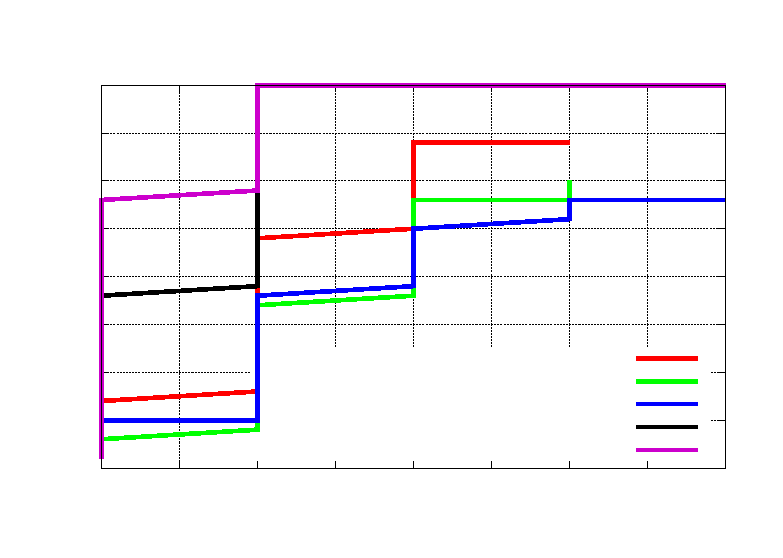
\includegraphics{plots/plot_2-2-3}}%
    \gplfronttext
  \end{picture}%
\endgroup

    \caption{Task 2.2.3: Comparison of f and HTL values for Rumor Mongering (40 peers)}
    \label{fig:2-2-3}
\end{figure}

\begin{figure}
    % GNUPLOT: LaTeX picture with Postscript
\begingroup
  \makeatletter
  \providecommand\color[2][]{%
    \GenericError{(gnuplot) \space\space\space\@spaces}{%
      Package color not loaded in conjunction with
      terminal option `colourtext'%
    }{See the gnuplot documentation for explanation.%
    }{Either use 'blacktext' in gnuplot or load the package
      color.sty in LaTeX.}%
    \renewcommand\color[2][]{}%
  }%
  \providecommand\includegraphics[2][]{%
    \GenericError{(gnuplot) \space\space\space\@spaces}{%
      Package graphicx or graphics not loaded%
    }{See the gnuplot documentation for explanation.%
    }{The gnuplot epslatex terminal needs graphicx.sty or graphics.sty.}%
    \renewcommand\includegraphics[2][]{}%
  }%
  \providecommand\rotatebox[2]{#2}%
  \@ifundefined{ifGPcolor}{%
    \newif\ifGPcolor
    \GPcolorfalse
  }{}%
  \@ifundefined{ifGPblacktext}{%
    \newif\ifGPblacktext
    \GPblacktexttrue
  }{}%
  % define a \g@addto@macro without @ in the name:
  \let\gplgaddtomacro\g@addto@macro
  % define empty templates for all commands taking text:
  \gdef\gplbacktext{}%
  \gdef\gplfronttext{}%
  \makeatother
  \ifGPblacktext
    % no textcolor at all
    \def\colorrgb#1{}%
    \def\colorgray#1{}%
  \else
    % gray or color?
    \ifGPcolor
      \def\colorrgb#1{\color[rgb]{#1}}%
      \def\colorgray#1{\color[gray]{#1}}%
      \expandafter\def\csname LTw\endcsname{\color{white}}%
      \expandafter\def\csname LTb\endcsname{\color{black}}%
      \expandafter\def\csname LTa\endcsname{\color{black}}%
      \expandafter\def\csname LT0\endcsname{\color[rgb]{1,0,0}}%
      \expandafter\def\csname LT1\endcsname{\color[rgb]{0,1,0}}%
      \expandafter\def\csname LT2\endcsname{\color[rgb]{0,0,1}}%
      \expandafter\def\csname LT3\endcsname{\color[rgb]{1,0,1}}%
      \expandafter\def\csname LT4\endcsname{\color[rgb]{0,1,1}}%
      \expandafter\def\csname LT5\endcsname{\color[rgb]{1,1,0}}%
      \expandafter\def\csname LT6\endcsname{\color[rgb]{0,0,0}}%
      \expandafter\def\csname LT7\endcsname{\color[rgb]{1,0.3,0}}%
      \expandafter\def\csname LT8\endcsname{\color[rgb]{0.5,0.5,0.5}}%
    \else
      % gray
      \def\colorrgb#1{\color{black}}%
      \def\colorgray#1{\color[gray]{#1}}%
      \expandafter\def\csname LTw\endcsname{\color{white}}%
      \expandafter\def\csname LTb\endcsname{\color{black}}%
      \expandafter\def\csname LTa\endcsname{\color{black}}%
      \expandafter\def\csname LT0\endcsname{\color{black}}%
      \expandafter\def\csname LT1\endcsname{\color{black}}%
      \expandafter\def\csname LT2\endcsname{\color{black}}%
      \expandafter\def\csname LT3\endcsname{\color{black}}%
      \expandafter\def\csname LT4\endcsname{\color{black}}%
      \expandafter\def\csname LT5\endcsname{\color{black}}%
      \expandafter\def\csname LT6\endcsname{\color{black}}%
      \expandafter\def\csname LT7\endcsname{\color{black}}%
      \expandafter\def\csname LT8\endcsname{\color{black}}%
    \fi
  \fi
    \setlength{\unitlength}{0.0500bp}%
    \ifx\gptboxheight\undefined%
      \newlength{\gptboxheight}%
      \newlength{\gptboxwidth}%
      \newsavebox{\gptboxtext}%
    \fi%
    \setlength{\fboxrule}{0.5pt}%
    \setlength{\fboxsep}{1pt}%
\begin{picture}(7200.00,5040.00)%
    \gplgaddtomacro\gplbacktext{%
      \csname LTb\endcsname%
      \put(682,704){\makebox(0,0)[r]{\strut{}$0$}}%
      \csname LTb\endcsname%
      \put(682,1163){\makebox(0,0)[r]{\strut{}$5$}}%
      \csname LTb\endcsname%
      \put(682,1623){\makebox(0,0)[r]{\strut{}$10$}}%
      \csname LTb\endcsname%
      \put(682,2082){\makebox(0,0)[r]{\strut{}$15$}}%
      \csname LTb\endcsname%
      \put(682,2542){\makebox(0,0)[r]{\strut{}$20$}}%
      \csname LTb\endcsname%
      \put(682,3001){\makebox(0,0)[r]{\strut{}$25$}}%
      \csname LTb\endcsname%
      \put(682,3460){\makebox(0,0)[r]{\strut{}$30$}}%
      \csname LTb\endcsname%
      \put(682,3920){\makebox(0,0)[r]{\strut{}$35$}}%
      \csname LTb\endcsname%
      \put(682,4379){\makebox(0,0)[r]{\strut{}$40$}}%
      \csname LTb\endcsname%
      \put(814,484){\makebox(0,0){\strut{}$0$}}%
      \csname LTb\endcsname%
      \put(2012,484){\makebox(0,0){\strut{}$5$}}%
      \csname LTb\endcsname%
      \put(3210,484){\makebox(0,0){\strut{}$10$}}%
      \csname LTb\endcsname%
      \put(4407,484){\makebox(0,0){\strut{}$15$}}%
      \csname LTb\endcsname%
      \put(5605,484){\makebox(0,0){\strut{}$20$}}%
      \csname LTb\endcsname%
      \put(6803,484){\makebox(0,0){\strut{}$25$}}%
    }%
    \gplgaddtomacro\gplfronttext{%
      \csname LTb\endcsname%
      \put(176,2541){\rotatebox{-270}{\makebox(0,0){\strut{}Peers Infected}}}%
      \put(3808,154){\makebox(0,0){\strut{}Seconds}}%
      \put(3808,4709){\makebox(0,0){\strut{}Rumor Mongering Dissemination}}%
      \csname LTb\endcsname%
      \put(5816,1757){\makebox(0,0)[r]{\strut{}HTL=4 f=3}}%
      \csname LTb\endcsname%
      \put(5816,1537){\makebox(0,0)[r]{\strut{}HTL=5 f=2}}%
      \csname LTb\endcsname%
      \put(5816,1317){\makebox(0,0)[r]{\strut{}HTL=5 f=3}}%
      \csname LTb\endcsname%
      \put(5816,1097){\makebox(0,0)[r]{\strut{}HTL=5 f=4}}%
      \csname LTb\endcsname%
      \put(5816,877){\makebox(0,0)[r]{\strut{}HTL=5 f=8}}%
    }%
    \gplbacktext
    \put(0,0){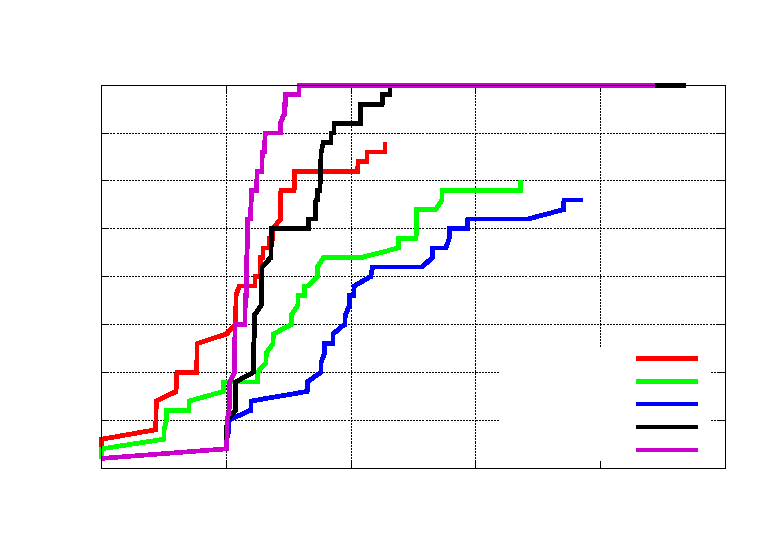
\includegraphics{plots/plot_2-2-3_seconds}}%
    \gplfronttext
  \end{picture}%
\endgroup

    \caption{Task 2.2.3: Comparison of f and HTL values for Rumor Mongering (40 peers)}
    \label{fig:2-2-3_seconds}
\end{figure}

Modyfing the initial\textunderscore hops\textunderscore to\textunderscore live and distribution\textunderscore count variables in the config section above, I examined some values of f and HTL. The results can be seen in figure \ref{fig:2-2-3}.

It seems to reach all my nodes, I need the parameter f to be at least 4 with HTL around 5.

For better readability, I also plotted the graph using seconds in the x axis. This plit is in figure \ref{fig:2-2-3_seconds}.

\section{Task 2.2.4}

The contained scripts parselog.lua and the various plot scrips are able to plot total infections and infections by type of infection. The log outputs both values, and the plot script decides which to plot.

\section{Task 2.3}

\begin{figure}
    % GNUPLOT: LaTeX picture with Postscript
\begingroup
  \makeatletter
  \providecommand\color[2][]{%
    \GenericError{(gnuplot) \space\space\space\@spaces}{%
      Package color not loaded in conjunction with
      terminal option `colourtext'%
    }{See the gnuplot documentation for explanation.%
    }{Either use 'blacktext' in gnuplot or load the package
      color.sty in LaTeX.}%
    \renewcommand\color[2][]{}%
  }%
  \providecommand\includegraphics[2][]{%
    \GenericError{(gnuplot) \space\space\space\@spaces}{%
      Package graphicx or graphics not loaded%
    }{See the gnuplot documentation for explanation.%
    }{The gnuplot epslatex terminal needs graphicx.sty or graphics.sty.}%
    \renewcommand\includegraphics[2][]{}%
  }%
  \providecommand\rotatebox[2]{#2}%
  \@ifundefined{ifGPcolor}{%
    \newif\ifGPcolor
    \GPcolorfalse
  }{}%
  \@ifundefined{ifGPblacktext}{%
    \newif\ifGPblacktext
    \GPblacktexttrue
  }{}%
  % define a \g@addto@macro without @ in the name:
  \let\gplgaddtomacro\g@addto@macro
  % define empty templates for all commands taking text:
  \gdef\gplbacktext{}%
  \gdef\gplfronttext{}%
  \makeatother
  \ifGPblacktext
    % no textcolor at all
    \def\colorrgb#1{}%
    \def\colorgray#1{}%
  \else
    % gray or color?
    \ifGPcolor
      \def\colorrgb#1{\color[rgb]{#1}}%
      \def\colorgray#1{\color[gray]{#1}}%
      \expandafter\def\csname LTw\endcsname{\color{white}}%
      \expandafter\def\csname LTb\endcsname{\color{black}}%
      \expandafter\def\csname LTa\endcsname{\color{black}}%
      \expandafter\def\csname LT0\endcsname{\color[rgb]{1,0,0}}%
      \expandafter\def\csname LT1\endcsname{\color[rgb]{0,1,0}}%
      \expandafter\def\csname LT2\endcsname{\color[rgb]{0,0,1}}%
      \expandafter\def\csname LT3\endcsname{\color[rgb]{1,0,1}}%
      \expandafter\def\csname LT4\endcsname{\color[rgb]{0,1,1}}%
      \expandafter\def\csname LT5\endcsname{\color[rgb]{1,1,0}}%
      \expandafter\def\csname LT6\endcsname{\color[rgb]{0,0,0}}%
      \expandafter\def\csname LT7\endcsname{\color[rgb]{1,0.3,0}}%
      \expandafter\def\csname LT8\endcsname{\color[rgb]{0.5,0.5,0.5}}%
    \else
      % gray
      \def\colorrgb#1{\color{black}}%
      \def\colorgray#1{\color[gray]{#1}}%
      \expandafter\def\csname LTw\endcsname{\color{white}}%
      \expandafter\def\csname LTb\endcsname{\color{black}}%
      \expandafter\def\csname LTa\endcsname{\color{black}}%
      \expandafter\def\csname LT0\endcsname{\color{black}}%
      \expandafter\def\csname LT1\endcsname{\color{black}}%
      \expandafter\def\csname LT2\endcsname{\color{black}}%
      \expandafter\def\csname LT3\endcsname{\color{black}}%
      \expandafter\def\csname LT4\endcsname{\color{black}}%
      \expandafter\def\csname LT5\endcsname{\color{black}}%
      \expandafter\def\csname LT6\endcsname{\color{black}}%
      \expandafter\def\csname LT7\endcsname{\color{black}}%
      \expandafter\def\csname LT8\endcsname{\color{black}}%
    \fi
  \fi
    \setlength{\unitlength}{0.0500bp}%
    \ifx\gptboxheight\undefined%
      \newlength{\gptboxheight}%
      \newlength{\gptboxwidth}%
      \newsavebox{\gptboxtext}%
    \fi%
    \setlength{\fboxrule}{0.5pt}%
    \setlength{\fboxsep}{1pt}%
\begin{picture}(7200.00,5040.00)%
    \gplgaddtomacro\gplbacktext{%
      \csname LTb\endcsname%
      \put(682,704){\makebox(0,0)[r]{\strut{}$0$}}%
      \csname LTb\endcsname%
      \put(682,1163){\makebox(0,0)[r]{\strut{}$5$}}%
      \csname LTb\endcsname%
      \put(682,1623){\makebox(0,0)[r]{\strut{}$10$}}%
      \csname LTb\endcsname%
      \put(682,2082){\makebox(0,0)[r]{\strut{}$15$}}%
      \csname LTb\endcsname%
      \put(682,2542){\makebox(0,0)[r]{\strut{}$20$}}%
      \csname LTb\endcsname%
      \put(682,3001){\makebox(0,0)[r]{\strut{}$25$}}%
      \csname LTb\endcsname%
      \put(682,3460){\makebox(0,0)[r]{\strut{}$30$}}%
      \csname LTb\endcsname%
      \put(682,3920){\makebox(0,0)[r]{\strut{}$35$}}%
      \csname LTb\endcsname%
      \put(682,4379){\makebox(0,0)[r]{\strut{}$40$}}%
      \csname LTb\endcsname%
      \put(814,484){\makebox(0,0){\strut{}$0$}}%
      \csname LTb\endcsname%
      \put(1812,484){\makebox(0,0){\strut{}$0.5$}}%
      \csname LTb\endcsname%
      \put(2810,484){\makebox(0,0){\strut{}$1$}}%
      \csname LTb\endcsname%
      \put(3809,484){\makebox(0,0){\strut{}$1.5$}}%
      \csname LTb\endcsname%
      \put(4807,484){\makebox(0,0){\strut{}$2$}}%
      \csname LTb\endcsname%
      \put(5805,484){\makebox(0,0){\strut{}$2.5$}}%
      \csname LTb\endcsname%
      \put(6803,484){\makebox(0,0){\strut{}$3$}}%
    }%
    \gplgaddtomacro\gplfronttext{%
      \csname LTb\endcsname%
      \put(176,2541){\rotatebox{-270}{\makebox(0,0){\strut{}Peers Infected}}}%
      \put(3808,154){\makebox(0,0){\strut{}Cycles}}%
      \put(3808,4709){\makebox(0,0){\strut{}Rumor Mongering and Anti-entropy comparison on 40 Peers.}}%
      \csname LTb\endcsname%
      \put(5816,1317){\makebox(0,0)[r]{\strut{}Total infections}}%
      \csname LTb\endcsname%
      \put(5816,1097){\makebox(0,0)[r]{\strut{}Infected by Anti-entropy}}%
      \csname LTb\endcsname%
      \put(5816,877){\makebox(0,0)[r]{\strut{}Infected by Rumor Mongering}}%
    }%
    \gplbacktext
    \put(0,0){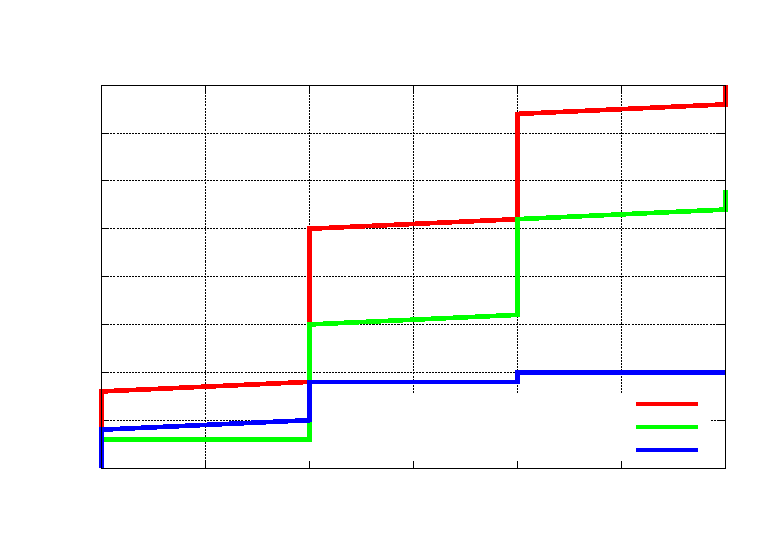
\includegraphics{plots/plot_2-3}}%
    \gplfronttext
  \end{picture}%
\endgroup

    \caption{Task 2.3: Comparison of Anti-entropy and Rumor Mongering on 40 peers}
    \label{fig:2-3}
\end{figure}

\begin{figure}
    % GNUPLOT: LaTeX picture with Postscript
\begingroup
  \makeatletter
  \providecommand\color[2][]{%
    \GenericError{(gnuplot) \space\space\space\@spaces}{%
      Package color not loaded in conjunction with
      terminal option `colourtext'%
    }{See the gnuplot documentation for explanation.%
    }{Either use 'blacktext' in gnuplot or load the package
      color.sty in LaTeX.}%
    \renewcommand\color[2][]{}%
  }%
  \providecommand\includegraphics[2][]{%
    \GenericError{(gnuplot) \space\space\space\@spaces}{%
      Package graphicx or graphics not loaded%
    }{See the gnuplot documentation for explanation.%
    }{The gnuplot epslatex terminal needs graphicx.sty or graphics.sty.}%
    \renewcommand\includegraphics[2][]{}%
  }%
  \providecommand\rotatebox[2]{#2}%
  \@ifundefined{ifGPcolor}{%
    \newif\ifGPcolor
    \GPcolorfalse
  }{}%
  \@ifundefined{ifGPblacktext}{%
    \newif\ifGPblacktext
    \GPblacktexttrue
  }{}%
  % define a \g@addto@macro without @ in the name:
  \let\gplgaddtomacro\g@addto@macro
  % define empty templates for all commands taking text:
  \gdef\gplbacktext{}%
  \gdef\gplfronttext{}%
  \makeatother
  \ifGPblacktext
    % no textcolor at all
    \def\colorrgb#1{}%
    \def\colorgray#1{}%
  \else
    % gray or color?
    \ifGPcolor
      \def\colorrgb#1{\color[rgb]{#1}}%
      \def\colorgray#1{\color[gray]{#1}}%
      \expandafter\def\csname LTw\endcsname{\color{white}}%
      \expandafter\def\csname LTb\endcsname{\color{black}}%
      \expandafter\def\csname LTa\endcsname{\color{black}}%
      \expandafter\def\csname LT0\endcsname{\color[rgb]{1,0,0}}%
      \expandafter\def\csname LT1\endcsname{\color[rgb]{0,1,0}}%
      \expandafter\def\csname LT2\endcsname{\color[rgb]{0,0,1}}%
      \expandafter\def\csname LT3\endcsname{\color[rgb]{1,0,1}}%
      \expandafter\def\csname LT4\endcsname{\color[rgb]{0,1,1}}%
      \expandafter\def\csname LT5\endcsname{\color[rgb]{1,1,0}}%
      \expandafter\def\csname LT6\endcsname{\color[rgb]{0,0,0}}%
      \expandafter\def\csname LT7\endcsname{\color[rgb]{1,0.3,0}}%
      \expandafter\def\csname LT8\endcsname{\color[rgb]{0.5,0.5,0.5}}%
    \else
      % gray
      \def\colorrgb#1{\color{black}}%
      \def\colorgray#1{\color[gray]{#1}}%
      \expandafter\def\csname LTw\endcsname{\color{white}}%
      \expandafter\def\csname LTb\endcsname{\color{black}}%
      \expandafter\def\csname LTa\endcsname{\color{black}}%
      \expandafter\def\csname LT0\endcsname{\color{black}}%
      \expandafter\def\csname LT1\endcsname{\color{black}}%
      \expandafter\def\csname LT2\endcsname{\color{black}}%
      \expandafter\def\csname LT3\endcsname{\color{black}}%
      \expandafter\def\csname LT4\endcsname{\color{black}}%
      \expandafter\def\csname LT5\endcsname{\color{black}}%
      \expandafter\def\csname LT6\endcsname{\color{black}}%
      \expandafter\def\csname LT7\endcsname{\color{black}}%
      \expandafter\def\csname LT8\endcsname{\color{black}}%
    \fi
  \fi
    \setlength{\unitlength}{0.0500bp}%
    \ifx\gptboxheight\undefined%
      \newlength{\gptboxheight}%
      \newlength{\gptboxwidth}%
      \newsavebox{\gptboxtext}%
    \fi%
    \setlength{\fboxrule}{0.5pt}%
    \setlength{\fboxsep}{1pt}%
\begin{picture}(7200.00,5040.00)%
    \gplgaddtomacro\gplbacktext{%
      \csname LTb\endcsname%
      \put(682,704){\makebox(0,0)[r]{\strut{}$0$}}%
      \csname LTb\endcsname%
      \put(682,1163){\makebox(0,0)[r]{\strut{}$5$}}%
      \csname LTb\endcsname%
      \put(682,1623){\makebox(0,0)[r]{\strut{}$10$}}%
      \csname LTb\endcsname%
      \put(682,2082){\makebox(0,0)[r]{\strut{}$15$}}%
      \csname LTb\endcsname%
      \put(682,2542){\makebox(0,0)[r]{\strut{}$20$}}%
      \csname LTb\endcsname%
      \put(682,3001){\makebox(0,0)[r]{\strut{}$25$}}%
      \csname LTb\endcsname%
      \put(682,3460){\makebox(0,0)[r]{\strut{}$30$}}%
      \csname LTb\endcsname%
      \put(682,3920){\makebox(0,0)[r]{\strut{}$35$}}%
      \csname LTb\endcsname%
      \put(682,4379){\makebox(0,0)[r]{\strut{}$40$}}%
      \csname LTb\endcsname%
      \put(814,484){\makebox(0,0){\strut{}$0$}}%
      \csname LTb\endcsname%
      \put(2311,484){\makebox(0,0){\strut{}$5$}}%
      \csname LTb\endcsname%
      \put(3809,484){\makebox(0,0){\strut{}$10$}}%
      \csname LTb\endcsname%
      \put(5306,484){\makebox(0,0){\strut{}$15$}}%
      \csname LTb\endcsname%
      \put(6803,484){\makebox(0,0){\strut{}$20$}}%
    }%
    \gplgaddtomacro\gplfronttext{%
      \csname LTb\endcsname%
      \put(176,2541){\rotatebox{-270}{\makebox(0,0){\strut{}Peers Infected}}}%
      \put(3808,154){\makebox(0,0){\strut{}Seconds}}%
      \put(3808,4709){\makebox(0,0){\strut{}Rumor Mongering and Anti-entropy comparison on 40 Peers.}}%
      \csname LTb\endcsname%
      \put(5816,1317){\makebox(0,0)[r]{\strut{}Total infections}}%
      \csname LTb\endcsname%
      \put(5816,1097){\makebox(0,0)[r]{\strut{}Infected by Anti-entropy}}%
      \csname LTb\endcsname%
      \put(5816,877){\makebox(0,0)[r]{\strut{}Infected by Rumor Mongering}}%
    }%
    \gplbacktext
    \put(0,0){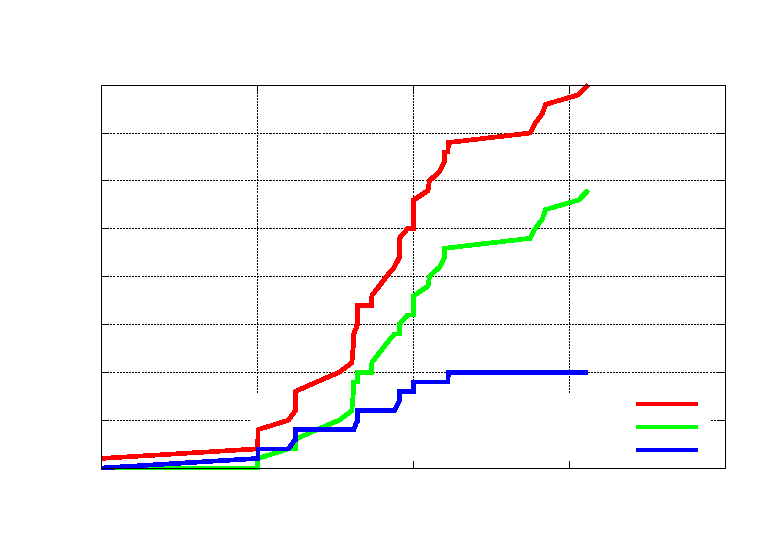
\includegraphics{plots/plot_2-3_seconds}}%
    \gplfronttext
  \end{picture}%
\endgroup

    \caption{Task 2.3: Comparison of Anti-entropy and Rumor Mongering on 40 peers}
    \label{fig:2-3_seconds}
\end{figure}

To show a comparison of the different infection methods, I use the following configuration:

\begin{lstlisting}
---START CONFIG SECTION---
do_rumor_mongering = true
do_anti_entropy = true
gossip_interval = 5
initial_hops_to_live = 3
distribution_count = 2
max_cycles = 20
start_gossipping_after_cycles = 0
---END CONFIG SECTION---
\end{lstlisting}

The resulting plot can be seen in figure \ref{fig:2-3}. There were 4 duplicates in the Rumor Mongering. I also plotted the graph with seconds in the x axis in figure \ref{fig:2-3_seconds}.

\section{Task 3.2}

I implemented the Peer Sampling Service in the gossip.lua file. I also wrote some unit tests for the array operations. To start gossip.lua in unit test mode, set the unit\textunderscore test\textunderscore mode constant to true. It will the run all the tests and end, and not actually start the simulation.

To use the Peer Sampling Service without any dissemination, I can use the following configuration:

\begin{lstlisting}
---START CONFIG SECTION---
do_peer_sampling = true
peer_sampling_interval = 5
peer_sampling_view_size = 8
peer_sampling_exchange_rate = 4
peer_sampling_healer_parameter = 1
peer_sampling_shuffler_parameter = 1
max_cycles = 10
---END CONFIG SECTION---
\end{lstlisting}

According to the check partion script, the graph is connected:

\lstinputlisting{logs/log_3-2_check_partition_output_h1s1.txt}

\begin{figure}
    % GNUPLOT: LaTeX picture with Postscript
\begingroup
  \makeatletter
  \providecommand\color[2][]{%
    \GenericError{(gnuplot) \space\space\space\@spaces}{%
      Package color not loaded in conjunction with
      terminal option `colourtext'%
    }{See the gnuplot documentation for explanation.%
    }{Either use 'blacktext' in gnuplot or load the package
      color.sty in LaTeX.}%
    \renewcommand\color[2][]{}%
  }%
  \providecommand\includegraphics[2][]{%
    \GenericError{(gnuplot) \space\space\space\@spaces}{%
      Package graphicx or graphics not loaded%
    }{See the gnuplot documentation for explanation.%
    }{The gnuplot epslatex terminal needs graphicx.sty or graphics.sty.}%
    \renewcommand\includegraphics[2][]{}%
  }%
  \providecommand\rotatebox[2]{#2}%
  \@ifundefined{ifGPcolor}{%
    \newif\ifGPcolor
    \GPcolorfalse
  }{}%
  \@ifundefined{ifGPblacktext}{%
    \newif\ifGPblacktext
    \GPblacktexttrue
  }{}%
  % define a \g@addto@macro without @ in the name:
  \let\gplgaddtomacro\g@addto@macro
  % define empty templates for all commands taking text:
  \gdef\gplbacktext{}%
  \gdef\gplfronttext{}%
  \makeatother
  \ifGPblacktext
    % no textcolor at all
    \def\colorrgb#1{}%
    \def\colorgray#1{}%
  \else
    % gray or color?
    \ifGPcolor
      \def\colorrgb#1{\color[rgb]{#1}}%
      \def\colorgray#1{\color[gray]{#1}}%
      \expandafter\def\csname LTw\endcsname{\color{white}}%
      \expandafter\def\csname LTb\endcsname{\color{black}}%
      \expandafter\def\csname LTa\endcsname{\color{black}}%
      \expandafter\def\csname LT0\endcsname{\color[rgb]{1,0,0}}%
      \expandafter\def\csname LT1\endcsname{\color[rgb]{0,1,0}}%
      \expandafter\def\csname LT2\endcsname{\color[rgb]{0,0,1}}%
      \expandafter\def\csname LT3\endcsname{\color[rgb]{1,0,1}}%
      \expandafter\def\csname LT4\endcsname{\color[rgb]{0,1,1}}%
      \expandafter\def\csname LT5\endcsname{\color[rgb]{1,1,0}}%
      \expandafter\def\csname LT6\endcsname{\color[rgb]{0,0,0}}%
      \expandafter\def\csname LT7\endcsname{\color[rgb]{1,0.3,0}}%
      \expandafter\def\csname LT8\endcsname{\color[rgb]{0.5,0.5,0.5}}%
    \else
      % gray
      \def\colorrgb#1{\color{black}}%
      \def\colorgray#1{\color[gray]{#1}}%
      \expandafter\def\csname LTw\endcsname{\color{white}}%
      \expandafter\def\csname LTb\endcsname{\color{black}}%
      \expandafter\def\csname LTa\endcsname{\color{black}}%
      \expandafter\def\csname LT0\endcsname{\color{black}}%
      \expandafter\def\csname LT1\endcsname{\color{black}}%
      \expandafter\def\csname LT2\endcsname{\color{black}}%
      \expandafter\def\csname LT3\endcsname{\color{black}}%
      \expandafter\def\csname LT4\endcsname{\color{black}}%
      \expandafter\def\csname LT5\endcsname{\color{black}}%
      \expandafter\def\csname LT6\endcsname{\color{black}}%
      \expandafter\def\csname LT7\endcsname{\color{black}}%
      \expandafter\def\csname LT8\endcsname{\color{black}}%
    \fi
  \fi
    \setlength{\unitlength}{0.0500bp}%
    \ifx\gptboxheight\undefined%
      \newlength{\gptboxheight}%
      \newlength{\gptboxwidth}%
      \newsavebox{\gptboxtext}%
    \fi%
    \setlength{\fboxrule}{0.5pt}%
    \setlength{\fboxsep}{1pt}%
\begin{picture}(7200.00,5040.00)%
    \gplgaddtomacro\gplbacktext{%
      \csname LTb\endcsname%
      \put(946,704){\makebox(0,0)[r]{\strut{}$0$}}%
      \csname LTb\endcsname%
      \put(946,1163){\makebox(0,0)[r]{\strut{}$0.05$}}%
      \csname LTb\endcsname%
      \put(946,1623){\makebox(0,0)[r]{\strut{}$0.1$}}%
      \csname LTb\endcsname%
      \put(946,2082){\makebox(0,0)[r]{\strut{}$0.15$}}%
      \csname LTb\endcsname%
      \put(946,2542){\makebox(0,0)[r]{\strut{}$0.2$}}%
      \csname LTb\endcsname%
      \put(946,3001){\makebox(0,0)[r]{\strut{}$0.25$}}%
      \csname LTb\endcsname%
      \put(946,3460){\makebox(0,0)[r]{\strut{}$0.3$}}%
      \csname LTb\endcsname%
      \put(946,3920){\makebox(0,0)[r]{\strut{}$0.35$}}%
      \csname LTb\endcsname%
      \put(946,4379){\makebox(0,0)[r]{\strut{}$0.4$}}%
      \csname LTb\endcsname%
      \put(1078,484){\makebox(0,0){\strut{}$0$}}%
      \csname LTb\endcsname%
      \put(2223,484){\makebox(0,0){\strut{}$10$}}%
      \csname LTb\endcsname%
      \put(3368,484){\makebox(0,0){\strut{}$20$}}%
      \csname LTb\endcsname%
      \put(4513,484){\makebox(0,0){\strut{}$30$}}%
      \csname LTb\endcsname%
      \put(5658,484){\makebox(0,0){\strut{}$40$}}%
      \csname LTb\endcsname%
      \put(6803,484){\makebox(0,0){\strut{}$50$}}%
    }%
    \gplgaddtomacro\gplfronttext{%
      \csname LTb\endcsname%
      \put(176,2541){\rotatebox{-270}{\makebox(0,0){\strut{}Clustering}}}%
      \put(3940,154){\makebox(0,0){\strut{}Peers (cumulated)}}%
      \put(3940,4709){\makebox(0,0){\strut{}Clustering Distribution for H=1 S=1}}%
    }%
    \gplbacktext
    \put(0,0){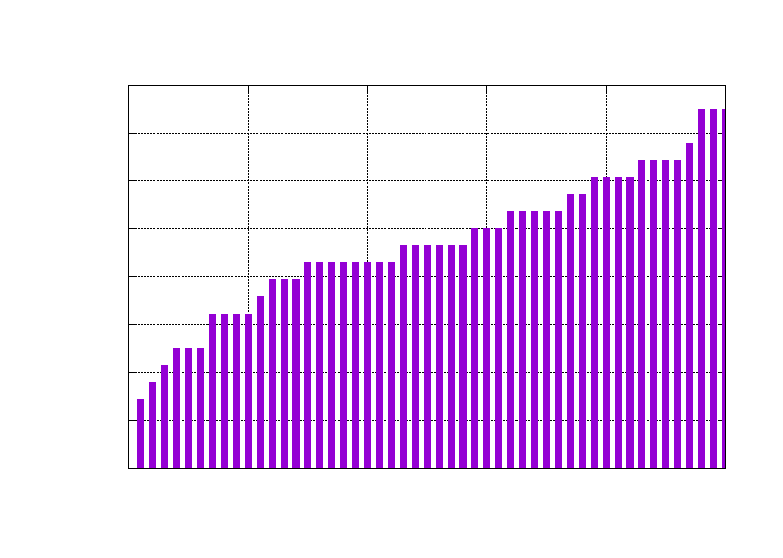
\includegraphics{plots/plot_3-2_h1s1_clustering}}%
    \gplfronttext
  \end{picture}%
\endgroup

    \caption{Task 3.2: Clustering (50 Peers, H=1, S=1)}
    \label{fig:3-2_h1s1_clustering}
\end{figure}

\begin{figure}
    % GNUPLOT: LaTeX picture with Postscript
\begingroup
  \makeatletter
  \providecommand\color[2][]{%
    \GenericError{(gnuplot) \space\space\space\@spaces}{%
      Package color not loaded in conjunction with
      terminal option `colourtext'%
    }{See the gnuplot documentation for explanation.%
    }{Either use 'blacktext' in gnuplot or load the package
      color.sty in LaTeX.}%
    \renewcommand\color[2][]{}%
  }%
  \providecommand\includegraphics[2][]{%
    \GenericError{(gnuplot) \space\space\space\@spaces}{%
      Package graphicx or graphics not loaded%
    }{See the gnuplot documentation for explanation.%
    }{The gnuplot epslatex terminal needs graphicx.sty or graphics.sty.}%
    \renewcommand\includegraphics[2][]{}%
  }%
  \providecommand\rotatebox[2]{#2}%
  \@ifundefined{ifGPcolor}{%
    \newif\ifGPcolor
    \GPcolorfalse
  }{}%
  \@ifundefined{ifGPblacktext}{%
    \newif\ifGPblacktext
    \GPblacktexttrue
  }{}%
  % define a \g@addto@macro without @ in the name:
  \let\gplgaddtomacro\g@addto@macro
  % define empty templates for all commands taking text:
  \gdef\gplbacktext{}%
  \gdef\gplfronttext{}%
  \makeatother
  \ifGPblacktext
    % no textcolor at all
    \def\colorrgb#1{}%
    \def\colorgray#1{}%
  \else
    % gray or color?
    \ifGPcolor
      \def\colorrgb#1{\color[rgb]{#1}}%
      \def\colorgray#1{\color[gray]{#1}}%
      \expandafter\def\csname LTw\endcsname{\color{white}}%
      \expandafter\def\csname LTb\endcsname{\color{black}}%
      \expandafter\def\csname LTa\endcsname{\color{black}}%
      \expandafter\def\csname LT0\endcsname{\color[rgb]{1,0,0}}%
      \expandafter\def\csname LT1\endcsname{\color[rgb]{0,1,0}}%
      \expandafter\def\csname LT2\endcsname{\color[rgb]{0,0,1}}%
      \expandafter\def\csname LT3\endcsname{\color[rgb]{1,0,1}}%
      \expandafter\def\csname LT4\endcsname{\color[rgb]{0,1,1}}%
      \expandafter\def\csname LT5\endcsname{\color[rgb]{1,1,0}}%
      \expandafter\def\csname LT6\endcsname{\color[rgb]{0,0,0}}%
      \expandafter\def\csname LT7\endcsname{\color[rgb]{1,0.3,0}}%
      \expandafter\def\csname LT8\endcsname{\color[rgb]{0.5,0.5,0.5}}%
    \else
      % gray
      \def\colorrgb#1{\color{black}}%
      \def\colorgray#1{\color[gray]{#1}}%
      \expandafter\def\csname LTw\endcsname{\color{white}}%
      \expandafter\def\csname LTb\endcsname{\color{black}}%
      \expandafter\def\csname LTa\endcsname{\color{black}}%
      \expandafter\def\csname LT0\endcsname{\color{black}}%
      \expandafter\def\csname LT1\endcsname{\color{black}}%
      \expandafter\def\csname LT2\endcsname{\color{black}}%
      \expandafter\def\csname LT3\endcsname{\color{black}}%
      \expandafter\def\csname LT4\endcsname{\color{black}}%
      \expandafter\def\csname LT5\endcsname{\color{black}}%
      \expandafter\def\csname LT6\endcsname{\color{black}}%
      \expandafter\def\csname LT7\endcsname{\color{black}}%
      \expandafter\def\csname LT8\endcsname{\color{black}}%
    \fi
  \fi
    \setlength{\unitlength}{0.0500bp}%
    \ifx\gptboxheight\undefined%
      \newlength{\gptboxheight}%
      \newlength{\gptboxwidth}%
      \newsavebox{\gptboxtext}%
    \fi%
    \setlength{\fboxrule}{0.5pt}%
    \setlength{\fboxsep}{1pt}%
\begin{picture}(7200.00,5040.00)%
    \gplgaddtomacro\gplbacktext{%
      \csname LTb\endcsname%
      \put(550,704){\makebox(0,0)[r]{\strut{}$0$}}%
      \csname LTb\endcsname%
      \put(550,1229){\makebox(0,0)[r]{\strut{}$1$}}%
      \csname LTb\endcsname%
      \put(550,1754){\makebox(0,0)[r]{\strut{}$2$}}%
      \csname LTb\endcsname%
      \put(550,2279){\makebox(0,0)[r]{\strut{}$3$}}%
      \csname LTb\endcsname%
      \put(550,2804){\makebox(0,0)[r]{\strut{}$4$}}%
      \csname LTb\endcsname%
      \put(550,3329){\makebox(0,0)[r]{\strut{}$5$}}%
      \csname LTb\endcsname%
      \put(550,3854){\makebox(0,0)[r]{\strut{}$6$}}%
      \csname LTb\endcsname%
      \put(550,4379){\makebox(0,0)[r]{\strut{}$7$}}%
      \csname LTb\endcsname%
      \put(682,484){\makebox(0,0){\strut{}$0$}}%
      \csname LTb\endcsname%
      \put(1294,484){\makebox(0,0){\strut{}$2$}}%
      \csname LTb\endcsname%
      \put(1906,484){\makebox(0,0){\strut{}$4$}}%
      \csname LTb\endcsname%
      \put(2518,484){\makebox(0,0){\strut{}$6$}}%
      \csname LTb\endcsname%
      \put(3130,484){\makebox(0,0){\strut{}$8$}}%
      \csname LTb\endcsname%
      \put(3743,484){\makebox(0,0){\strut{}$10$}}%
      \csname LTb\endcsname%
      \put(4355,484){\makebox(0,0){\strut{}$12$}}%
      \csname LTb\endcsname%
      \put(4967,484){\makebox(0,0){\strut{}$14$}}%
      \csname LTb\endcsname%
      \put(5579,484){\makebox(0,0){\strut{}$16$}}%
      \csname LTb\endcsname%
      \put(6191,484){\makebox(0,0){\strut{}$18$}}%
      \csname LTb\endcsname%
      \put(6803,484){\makebox(0,0){\strut{}$20$}}%
    }%
    \gplgaddtomacro\gplfronttext{%
      \csname LTb\endcsname%
      \put(176,2541){\rotatebox{-270}{\makebox(0,0){\strut{}Number of Nodes}}}%
      \put(3742,154){\makebox(0,0){\strut{}In-Degree}}%
      \put(3742,4709){\makebox(0,0){\strut{}In-degree Distribution for H=1 S=1}}%
    }%
    \gplbacktext
    \put(0,0){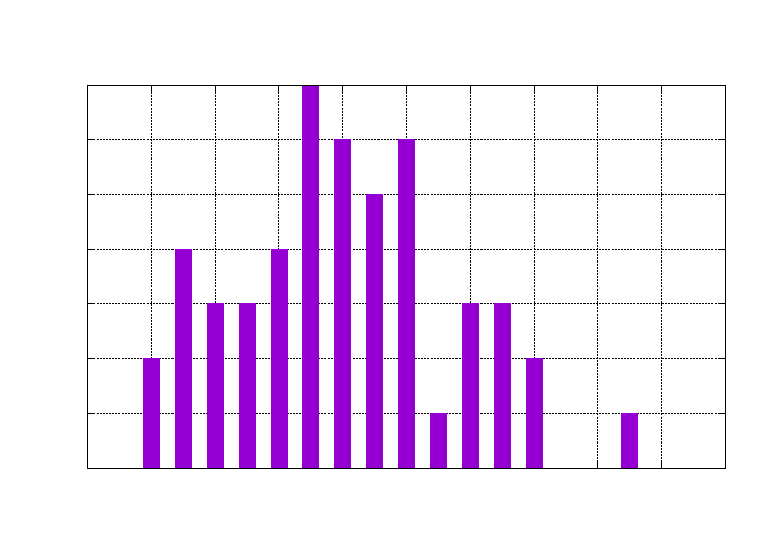
\includegraphics{plots/plot_3-2_h1s1_indegrees}}%
    \gplfronttext
  \end{picture}%
\endgroup

    \caption{Task 3.2: In-degrees (50 Peers, H=1, S=1)}
    \label{fig:3-2_h1s1_indegrees}
\end{figure}

\begin{figure}
    % GNUPLOT: LaTeX picture with Postscript
\begingroup
  \makeatletter
  \providecommand\color[2][]{%
    \GenericError{(gnuplot) \space\space\space\@spaces}{%
      Package color not loaded in conjunction with
      terminal option `colourtext'%
    }{See the gnuplot documentation for explanation.%
    }{Either use 'blacktext' in gnuplot or load the package
      color.sty in LaTeX.}%
    \renewcommand\color[2][]{}%
  }%
  \providecommand\includegraphics[2][]{%
    \GenericError{(gnuplot) \space\space\space\@spaces}{%
      Package graphicx or graphics not loaded%
    }{See the gnuplot documentation for explanation.%
    }{The gnuplot epslatex terminal needs graphicx.sty or graphics.sty.}%
    \renewcommand\includegraphics[2][]{}%
  }%
  \providecommand\rotatebox[2]{#2}%
  \@ifundefined{ifGPcolor}{%
    \newif\ifGPcolor
    \GPcolorfalse
  }{}%
  \@ifundefined{ifGPblacktext}{%
    \newif\ifGPblacktext
    \GPblacktexttrue
  }{}%
  % define a \g@addto@macro without @ in the name:
  \let\gplgaddtomacro\g@addto@macro
  % define empty templates for all commands taking text:
  \gdef\gplbacktext{}%
  \gdef\gplfronttext{}%
  \makeatother
  \ifGPblacktext
    % no textcolor at all
    \def\colorrgb#1{}%
    \def\colorgray#1{}%
  \else
    % gray or color?
    \ifGPcolor
      \def\colorrgb#1{\color[rgb]{#1}}%
      \def\colorgray#1{\color[gray]{#1}}%
      \expandafter\def\csname LTw\endcsname{\color{white}}%
      \expandafter\def\csname LTb\endcsname{\color{black}}%
      \expandafter\def\csname LTa\endcsname{\color{black}}%
      \expandafter\def\csname LT0\endcsname{\color[rgb]{1,0,0}}%
      \expandafter\def\csname LT1\endcsname{\color[rgb]{0,1,0}}%
      \expandafter\def\csname LT2\endcsname{\color[rgb]{0,0,1}}%
      \expandafter\def\csname LT3\endcsname{\color[rgb]{1,0,1}}%
      \expandafter\def\csname LT4\endcsname{\color[rgb]{0,1,1}}%
      \expandafter\def\csname LT5\endcsname{\color[rgb]{1,1,0}}%
      \expandafter\def\csname LT6\endcsname{\color[rgb]{0,0,0}}%
      \expandafter\def\csname LT7\endcsname{\color[rgb]{1,0.3,0}}%
      \expandafter\def\csname LT8\endcsname{\color[rgb]{0.5,0.5,0.5}}%
    \else
      % gray
      \def\colorrgb#1{\color{black}}%
      \def\colorgray#1{\color[gray]{#1}}%
      \expandafter\def\csname LTw\endcsname{\color{white}}%
      \expandafter\def\csname LTb\endcsname{\color{black}}%
      \expandafter\def\csname LTa\endcsname{\color{black}}%
      \expandafter\def\csname LT0\endcsname{\color{black}}%
      \expandafter\def\csname LT1\endcsname{\color{black}}%
      \expandafter\def\csname LT2\endcsname{\color{black}}%
      \expandafter\def\csname LT3\endcsname{\color{black}}%
      \expandafter\def\csname LT4\endcsname{\color{black}}%
      \expandafter\def\csname LT5\endcsname{\color{black}}%
      \expandafter\def\csname LT6\endcsname{\color{black}}%
      \expandafter\def\csname LT7\endcsname{\color{black}}%
      \expandafter\def\csname LT8\endcsname{\color{black}}%
    \fi
  \fi
    \setlength{\unitlength}{0.0500bp}%
    \ifx\gptboxheight\undefined%
      \newlength{\gptboxheight}%
      \newlength{\gptboxwidth}%
      \newsavebox{\gptboxtext}%
    \fi%
    \setlength{\fboxrule}{0.5pt}%
    \setlength{\fboxsep}{1pt}%
\begin{picture}(7200.00,5040.00)%
    \gplgaddtomacro\gplbacktext{%
      \csname LTb\endcsname%
      \put(946,704){\makebox(0,0)[r]{\strut{}$0$}}%
      \csname LTb\endcsname%
      \put(946,1112){\makebox(0,0)[r]{\strut{}$0.05$}}%
      \csname LTb\endcsname%
      \put(946,1521){\makebox(0,0)[r]{\strut{}$0.1$}}%
      \csname LTb\endcsname%
      \put(946,1929){\makebox(0,0)[r]{\strut{}$0.15$}}%
      \csname LTb\endcsname%
      \put(946,2337){\makebox(0,0)[r]{\strut{}$0.2$}}%
      \csname LTb\endcsname%
      \put(946,2746){\makebox(0,0)[r]{\strut{}$0.25$}}%
      \csname LTb\endcsname%
      \put(946,3154){\makebox(0,0)[r]{\strut{}$0.3$}}%
      \csname LTb\endcsname%
      \put(946,3562){\makebox(0,0)[r]{\strut{}$0.35$}}%
      \csname LTb\endcsname%
      \put(946,3971){\makebox(0,0)[r]{\strut{}$0.4$}}%
      \csname LTb\endcsname%
      \put(946,4379){\makebox(0,0)[r]{\strut{}$0.45$}}%
      \csname LTb\endcsname%
      \put(1078,484){\makebox(0,0){\strut{}$0$}}%
      \csname LTb\endcsname%
      \put(2223,484){\makebox(0,0){\strut{}$10$}}%
      \csname LTb\endcsname%
      \put(3368,484){\makebox(0,0){\strut{}$20$}}%
      \csname LTb\endcsname%
      \put(4513,484){\makebox(0,0){\strut{}$30$}}%
      \csname LTb\endcsname%
      \put(5658,484){\makebox(0,0){\strut{}$40$}}%
      \csname LTb\endcsname%
      \put(6803,484){\makebox(0,0){\strut{}$50$}}%
    }%
    \gplgaddtomacro\gplfronttext{%
      \csname LTb\endcsname%
      \put(176,2541){\rotatebox{-270}{\makebox(0,0){\strut{}Clustering}}}%
      \put(3940,154){\makebox(0,0){\strut{}Peers (cumulated)}}%
      \put(3940,4709){\makebox(0,0){\strut{}Clustering Distribution for H=0 S=0}}%
    }%
    \gplbacktext
    \put(0,0){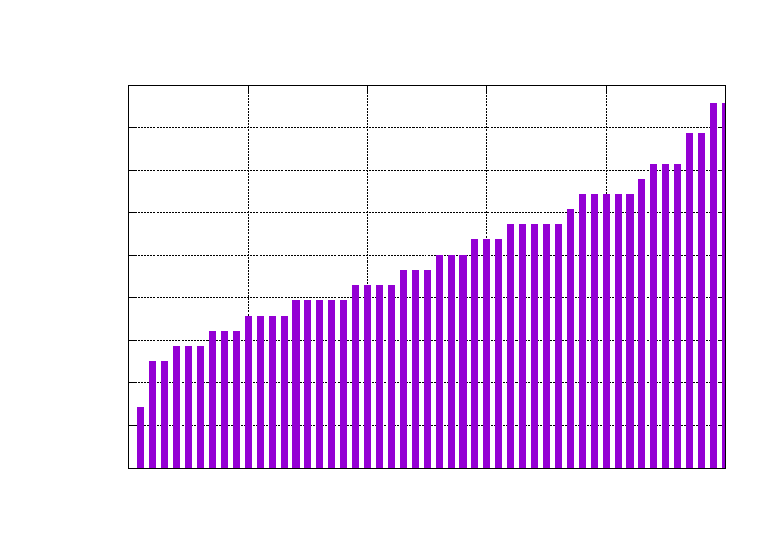
\includegraphics{plots/plot_3-2_h0s0_clustering}}%
    \gplfronttext
  \end{picture}%
\endgroup

    \caption{Task 3.2: Clustering (50 Peers, H=0, S=0)}
    \label{fig:3-2_h0s0_clustering}
\end{figure}

\begin{figure}
    % GNUPLOT: LaTeX picture with Postscript
\begingroup
  \makeatletter
  \providecommand\color[2][]{%
    \GenericError{(gnuplot) \space\space\space\@spaces}{%
      Package color not loaded in conjunction with
      terminal option `colourtext'%
    }{See the gnuplot documentation for explanation.%
    }{Either use 'blacktext' in gnuplot or load the package
      color.sty in LaTeX.}%
    \renewcommand\color[2][]{}%
  }%
  \providecommand\includegraphics[2][]{%
    \GenericError{(gnuplot) \space\space\space\@spaces}{%
      Package graphicx or graphics not loaded%
    }{See the gnuplot documentation for explanation.%
    }{The gnuplot epslatex terminal needs graphicx.sty or graphics.sty.}%
    \renewcommand\includegraphics[2][]{}%
  }%
  \providecommand\rotatebox[2]{#2}%
  \@ifundefined{ifGPcolor}{%
    \newif\ifGPcolor
    \GPcolorfalse
  }{}%
  \@ifundefined{ifGPblacktext}{%
    \newif\ifGPblacktext
    \GPblacktexttrue
  }{}%
  % define a \g@addto@macro without @ in the name:
  \let\gplgaddtomacro\g@addto@macro
  % define empty templates for all commands taking text:
  \gdef\gplbacktext{}%
  \gdef\gplfronttext{}%
  \makeatother
  \ifGPblacktext
    % no textcolor at all
    \def\colorrgb#1{}%
    \def\colorgray#1{}%
  \else
    % gray or color?
    \ifGPcolor
      \def\colorrgb#1{\color[rgb]{#1}}%
      \def\colorgray#1{\color[gray]{#1}}%
      \expandafter\def\csname LTw\endcsname{\color{white}}%
      \expandafter\def\csname LTb\endcsname{\color{black}}%
      \expandafter\def\csname LTa\endcsname{\color{black}}%
      \expandafter\def\csname LT0\endcsname{\color[rgb]{1,0,0}}%
      \expandafter\def\csname LT1\endcsname{\color[rgb]{0,1,0}}%
      \expandafter\def\csname LT2\endcsname{\color[rgb]{0,0,1}}%
      \expandafter\def\csname LT3\endcsname{\color[rgb]{1,0,1}}%
      \expandafter\def\csname LT4\endcsname{\color[rgb]{0,1,1}}%
      \expandafter\def\csname LT5\endcsname{\color[rgb]{1,1,0}}%
      \expandafter\def\csname LT6\endcsname{\color[rgb]{0,0,0}}%
      \expandafter\def\csname LT7\endcsname{\color[rgb]{1,0.3,0}}%
      \expandafter\def\csname LT8\endcsname{\color[rgb]{0.5,0.5,0.5}}%
    \else
      % gray
      \def\colorrgb#1{\color{black}}%
      \def\colorgray#1{\color[gray]{#1}}%
      \expandafter\def\csname LTw\endcsname{\color{white}}%
      \expandafter\def\csname LTb\endcsname{\color{black}}%
      \expandafter\def\csname LTa\endcsname{\color{black}}%
      \expandafter\def\csname LT0\endcsname{\color{black}}%
      \expandafter\def\csname LT1\endcsname{\color{black}}%
      \expandafter\def\csname LT2\endcsname{\color{black}}%
      \expandafter\def\csname LT3\endcsname{\color{black}}%
      \expandafter\def\csname LT4\endcsname{\color{black}}%
      \expandafter\def\csname LT5\endcsname{\color{black}}%
      \expandafter\def\csname LT6\endcsname{\color{black}}%
      \expandafter\def\csname LT7\endcsname{\color{black}}%
      \expandafter\def\csname LT8\endcsname{\color{black}}%
    \fi
  \fi
    \setlength{\unitlength}{0.0500bp}%
    \ifx\gptboxheight\undefined%
      \newlength{\gptboxheight}%
      \newlength{\gptboxwidth}%
      \newsavebox{\gptboxtext}%
    \fi%
    \setlength{\fboxrule}{0.5pt}%
    \setlength{\fboxsep}{1pt}%
\begin{picture}(7200.00,5040.00)%
    \gplgaddtomacro\gplbacktext{%
      \csname LTb\endcsname%
      \put(550,704){\makebox(0,0)[r]{\strut{}$0$}}%
      \csname LTb\endcsname%
      \put(550,1163){\makebox(0,0)[r]{\strut{}$1$}}%
      \csname LTb\endcsname%
      \put(550,1623){\makebox(0,0)[r]{\strut{}$2$}}%
      \csname LTb\endcsname%
      \put(550,2082){\makebox(0,0)[r]{\strut{}$3$}}%
      \csname LTb\endcsname%
      \put(550,2542){\makebox(0,0)[r]{\strut{}$4$}}%
      \csname LTb\endcsname%
      \put(550,3001){\makebox(0,0)[r]{\strut{}$5$}}%
      \csname LTb\endcsname%
      \put(550,3460){\makebox(0,0)[r]{\strut{}$6$}}%
      \csname LTb\endcsname%
      \put(550,3920){\makebox(0,0)[r]{\strut{}$7$}}%
      \csname LTb\endcsname%
      \put(550,4379){\makebox(0,0)[r]{\strut{}$8$}}%
      \csname LTb\endcsname%
      \put(682,484){\makebox(0,0){\strut{}$0$}}%
      \csname LTb\endcsname%
      \put(1447,484){\makebox(0,0){\strut{}$2$}}%
      \csname LTb\endcsname%
      \put(2212,484){\makebox(0,0){\strut{}$4$}}%
      \csname LTb\endcsname%
      \put(2977,484){\makebox(0,0){\strut{}$6$}}%
      \csname LTb\endcsname%
      \put(3743,484){\makebox(0,0){\strut{}$8$}}%
      \csname LTb\endcsname%
      \put(4508,484){\makebox(0,0){\strut{}$10$}}%
      \csname LTb\endcsname%
      \put(5273,484){\makebox(0,0){\strut{}$12$}}%
      \csname LTb\endcsname%
      \put(6038,484){\makebox(0,0){\strut{}$14$}}%
      \csname LTb\endcsname%
      \put(6803,484){\makebox(0,0){\strut{}$16$}}%
    }%
    \gplgaddtomacro\gplfronttext{%
      \csname LTb\endcsname%
      \put(176,2541){\rotatebox{-270}{\makebox(0,0){\strut{}Number of Nodes}}}%
      \put(3742,154){\makebox(0,0){\strut{}In-Degree}}%
      \put(3742,4709){\makebox(0,0){\strut{}In-degree Distribution for H=0 S=0}}%
    }%
    \gplbacktext
    \put(0,0){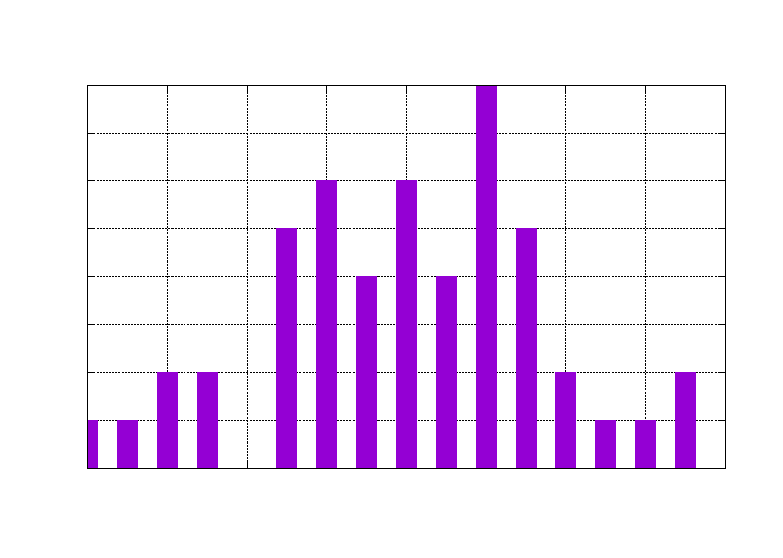
\includegraphics{plots/plot_3-2_h0s0_indegrees}}%
    \gplfronttext
  \end{picture}%
\endgroup

    \caption{Task 3.2: In-degrees (50 Peers, H=0, S=0)}
    \label{fig:3-2_h0s0_indegrees}
\end{figure}

\begin{figure}
    % GNUPLOT: LaTeX picture with Postscript
\begingroup
  \makeatletter
  \providecommand\color[2][]{%
    \GenericError{(gnuplot) \space\space\space\@spaces}{%
      Package color not loaded in conjunction with
      terminal option `colourtext'%
    }{See the gnuplot documentation for explanation.%
    }{Either use 'blacktext' in gnuplot or load the package
      color.sty in LaTeX.}%
    \renewcommand\color[2][]{}%
  }%
  \providecommand\includegraphics[2][]{%
    \GenericError{(gnuplot) \space\space\space\@spaces}{%
      Package graphicx or graphics not loaded%
    }{See the gnuplot documentation for explanation.%
    }{The gnuplot epslatex terminal needs graphicx.sty or graphics.sty.}%
    \renewcommand\includegraphics[2][]{}%
  }%
  \providecommand\rotatebox[2]{#2}%
  \@ifundefined{ifGPcolor}{%
    \newif\ifGPcolor
    \GPcolorfalse
  }{}%
  \@ifundefined{ifGPblacktext}{%
    \newif\ifGPblacktext
    \GPblacktexttrue
  }{}%
  % define a \g@addto@macro without @ in the name:
  \let\gplgaddtomacro\g@addto@macro
  % define empty templates for all commands taking text:
  \gdef\gplbacktext{}%
  \gdef\gplfronttext{}%
  \makeatother
  \ifGPblacktext
    % no textcolor at all
    \def\colorrgb#1{}%
    \def\colorgray#1{}%
  \else
    % gray or color?
    \ifGPcolor
      \def\colorrgb#1{\color[rgb]{#1}}%
      \def\colorgray#1{\color[gray]{#1}}%
      \expandafter\def\csname LTw\endcsname{\color{white}}%
      \expandafter\def\csname LTb\endcsname{\color{black}}%
      \expandafter\def\csname LTa\endcsname{\color{black}}%
      \expandafter\def\csname LT0\endcsname{\color[rgb]{1,0,0}}%
      \expandafter\def\csname LT1\endcsname{\color[rgb]{0,1,0}}%
      \expandafter\def\csname LT2\endcsname{\color[rgb]{0,0,1}}%
      \expandafter\def\csname LT3\endcsname{\color[rgb]{1,0,1}}%
      \expandafter\def\csname LT4\endcsname{\color[rgb]{0,1,1}}%
      \expandafter\def\csname LT5\endcsname{\color[rgb]{1,1,0}}%
      \expandafter\def\csname LT6\endcsname{\color[rgb]{0,0,0}}%
      \expandafter\def\csname LT7\endcsname{\color[rgb]{1,0.3,0}}%
      \expandafter\def\csname LT8\endcsname{\color[rgb]{0.5,0.5,0.5}}%
    \else
      % gray
      \def\colorrgb#1{\color{black}}%
      \def\colorgray#1{\color[gray]{#1}}%
      \expandafter\def\csname LTw\endcsname{\color{white}}%
      \expandafter\def\csname LTb\endcsname{\color{black}}%
      \expandafter\def\csname LTa\endcsname{\color{black}}%
      \expandafter\def\csname LT0\endcsname{\color{black}}%
      \expandafter\def\csname LT1\endcsname{\color{black}}%
      \expandafter\def\csname LT2\endcsname{\color{black}}%
      \expandafter\def\csname LT3\endcsname{\color{black}}%
      \expandafter\def\csname LT4\endcsname{\color{black}}%
      \expandafter\def\csname LT5\endcsname{\color{black}}%
      \expandafter\def\csname LT6\endcsname{\color{black}}%
      \expandafter\def\csname LT7\endcsname{\color{black}}%
      \expandafter\def\csname LT8\endcsname{\color{black}}%
    \fi
  \fi
    \setlength{\unitlength}{0.0500bp}%
    \ifx\gptboxheight\undefined%
      \newlength{\gptboxheight}%
      \newlength{\gptboxwidth}%
      \newsavebox{\gptboxtext}%
    \fi%
    \setlength{\fboxrule}{0.5pt}%
    \setlength{\fboxsep}{1pt}%
\begin{picture}(7200.00,5040.00)%
    \gplgaddtomacro\gplbacktext{%
      \csname LTb\endcsname%
      \put(814,704){\makebox(0,0)[r]{\strut{}$0$}}%
      \csname LTb\endcsname%
      \put(814,1317){\makebox(0,0)[r]{\strut{}$0.1$}}%
      \csname LTb\endcsname%
      \put(814,1929){\makebox(0,0)[r]{\strut{}$0.2$}}%
      \csname LTb\endcsname%
      \put(814,2542){\makebox(0,0)[r]{\strut{}$0.3$}}%
      \csname LTb\endcsname%
      \put(814,3154){\makebox(0,0)[r]{\strut{}$0.4$}}%
      \csname LTb\endcsname%
      \put(814,3766){\makebox(0,0)[r]{\strut{}$0.5$}}%
      \csname LTb\endcsname%
      \put(814,4379){\makebox(0,0)[r]{\strut{}$0.6$}}%
      \csname LTb\endcsname%
      \put(946,484){\makebox(0,0){\strut{}$0$}}%
      \csname LTb\endcsname%
      \put(2117,484){\makebox(0,0){\strut{}$10$}}%
      \csname LTb\endcsname%
      \put(3289,484){\makebox(0,0){\strut{}$20$}}%
      \csname LTb\endcsname%
      \put(4460,484){\makebox(0,0){\strut{}$30$}}%
      \csname LTb\endcsname%
      \put(5632,484){\makebox(0,0){\strut{}$40$}}%
      \csname LTb\endcsname%
      \put(6803,484){\makebox(0,0){\strut{}$50$}}%
    }%
    \gplgaddtomacro\gplfronttext{%
      \csname LTb\endcsname%
      \put(176,2541){\rotatebox{-270}{\makebox(0,0){\strut{}Clustering}}}%
      \put(3874,154){\makebox(0,0){\strut{}Peers (cumulated)}}%
      \put(3874,4709){\makebox(0,0){\strut{}Clustering Distribution for H=4 S=0}}%
    }%
    \gplbacktext
    \put(0,0){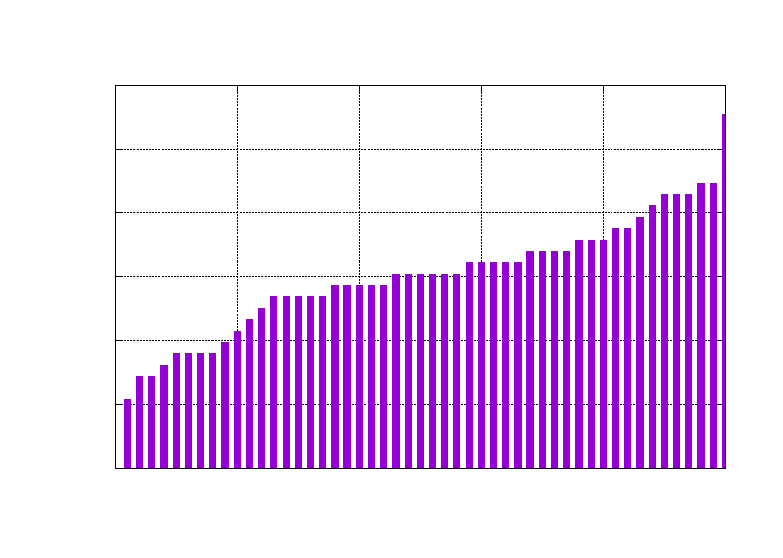
\includegraphics{plots/plot_3-2_h4s0_clustering}}%
    \gplfronttext
  \end{picture}%
\endgroup

    \caption{Task 3.2: Clustering (50 Peers, H=4, S=0)}
    \label{fig:3-2_h4s0_clustering}
\end{figure}

\begin{figure}
    % GNUPLOT: LaTeX picture with Postscript
\begingroup
  \makeatletter
  \providecommand\color[2][]{%
    \GenericError{(gnuplot) \space\space\space\@spaces}{%
      Package color not loaded in conjunction with
      terminal option `colourtext'%
    }{See the gnuplot documentation for explanation.%
    }{Either use 'blacktext' in gnuplot or load the package
      color.sty in LaTeX.}%
    \renewcommand\color[2][]{}%
  }%
  \providecommand\includegraphics[2][]{%
    \GenericError{(gnuplot) \space\space\space\@spaces}{%
      Package graphicx or graphics not loaded%
    }{See the gnuplot documentation for explanation.%
    }{The gnuplot epslatex terminal needs graphicx.sty or graphics.sty.}%
    \renewcommand\includegraphics[2][]{}%
  }%
  \providecommand\rotatebox[2]{#2}%
  \@ifundefined{ifGPcolor}{%
    \newif\ifGPcolor
    \GPcolorfalse
  }{}%
  \@ifundefined{ifGPblacktext}{%
    \newif\ifGPblacktext
    \GPblacktexttrue
  }{}%
  % define a \g@addto@macro without @ in the name:
  \let\gplgaddtomacro\g@addto@macro
  % define empty templates for all commands taking text:
  \gdef\gplbacktext{}%
  \gdef\gplfronttext{}%
  \makeatother
  \ifGPblacktext
    % no textcolor at all
    \def\colorrgb#1{}%
    \def\colorgray#1{}%
  \else
    % gray or color?
    \ifGPcolor
      \def\colorrgb#1{\color[rgb]{#1}}%
      \def\colorgray#1{\color[gray]{#1}}%
      \expandafter\def\csname LTw\endcsname{\color{white}}%
      \expandafter\def\csname LTb\endcsname{\color{black}}%
      \expandafter\def\csname LTa\endcsname{\color{black}}%
      \expandafter\def\csname LT0\endcsname{\color[rgb]{1,0,0}}%
      \expandafter\def\csname LT1\endcsname{\color[rgb]{0,1,0}}%
      \expandafter\def\csname LT2\endcsname{\color[rgb]{0,0,1}}%
      \expandafter\def\csname LT3\endcsname{\color[rgb]{1,0,1}}%
      \expandafter\def\csname LT4\endcsname{\color[rgb]{0,1,1}}%
      \expandafter\def\csname LT5\endcsname{\color[rgb]{1,1,0}}%
      \expandafter\def\csname LT6\endcsname{\color[rgb]{0,0,0}}%
      \expandafter\def\csname LT7\endcsname{\color[rgb]{1,0.3,0}}%
      \expandafter\def\csname LT8\endcsname{\color[rgb]{0.5,0.5,0.5}}%
    \else
      % gray
      \def\colorrgb#1{\color{black}}%
      \def\colorgray#1{\color[gray]{#1}}%
      \expandafter\def\csname LTw\endcsname{\color{white}}%
      \expandafter\def\csname LTb\endcsname{\color{black}}%
      \expandafter\def\csname LTa\endcsname{\color{black}}%
      \expandafter\def\csname LT0\endcsname{\color{black}}%
      \expandafter\def\csname LT1\endcsname{\color{black}}%
      \expandafter\def\csname LT2\endcsname{\color{black}}%
      \expandafter\def\csname LT3\endcsname{\color{black}}%
      \expandafter\def\csname LT4\endcsname{\color{black}}%
      \expandafter\def\csname LT5\endcsname{\color{black}}%
      \expandafter\def\csname LT6\endcsname{\color{black}}%
      \expandafter\def\csname LT7\endcsname{\color{black}}%
      \expandafter\def\csname LT8\endcsname{\color{black}}%
    \fi
  \fi
    \setlength{\unitlength}{0.0500bp}%
    \ifx\gptboxheight\undefined%
      \newlength{\gptboxheight}%
      \newlength{\gptboxwidth}%
      \newsavebox{\gptboxtext}%
    \fi%
    \setlength{\fboxrule}{0.5pt}%
    \setlength{\fboxsep}{1pt}%
\begin{picture}(7200.00,5040.00)%
    \gplgaddtomacro\gplbacktext{%
      \csname LTb\endcsname%
      \put(550,704){\makebox(0,0)[r]{\strut{}$0$}}%
      \csname LTb\endcsname%
      \put(550,1163){\makebox(0,0)[r]{\strut{}$1$}}%
      \csname LTb\endcsname%
      \put(550,1623){\makebox(0,0)[r]{\strut{}$2$}}%
      \csname LTb\endcsname%
      \put(550,2082){\makebox(0,0)[r]{\strut{}$3$}}%
      \csname LTb\endcsname%
      \put(550,2542){\makebox(0,0)[r]{\strut{}$4$}}%
      \csname LTb\endcsname%
      \put(550,3001){\makebox(0,0)[r]{\strut{}$5$}}%
      \csname LTb\endcsname%
      \put(550,3460){\makebox(0,0)[r]{\strut{}$6$}}%
      \csname LTb\endcsname%
      \put(550,3920){\makebox(0,0)[r]{\strut{}$7$}}%
      \csname LTb\endcsname%
      \put(550,4379){\makebox(0,0)[r]{\strut{}$8$}}%
      \csname LTb\endcsname%
      \put(682,484){\makebox(0,0){\strut{}$0$}}%
      \csname LTb\endcsname%
      \put(1906,484){\makebox(0,0){\strut{}$5$}}%
      \csname LTb\endcsname%
      \put(3130,484){\makebox(0,0){\strut{}$10$}}%
      \csname LTb\endcsname%
      \put(4355,484){\makebox(0,0){\strut{}$15$}}%
      \csname LTb\endcsname%
      \put(5579,484){\makebox(0,0){\strut{}$20$}}%
      \csname LTb\endcsname%
      \put(6803,484){\makebox(0,0){\strut{}$25$}}%
    }%
    \gplgaddtomacro\gplfronttext{%
      \csname LTb\endcsname%
      \put(176,2541){\rotatebox{-270}{\makebox(0,0){\strut{}Number of Nodes}}}%
      \put(3742,154){\makebox(0,0){\strut{}In-Degree}}%
      \put(3742,4709){\makebox(0,0){\strut{}In-degree Distribution for H=4 S=0}}%
    }%
    \gplbacktext
    \put(0,0){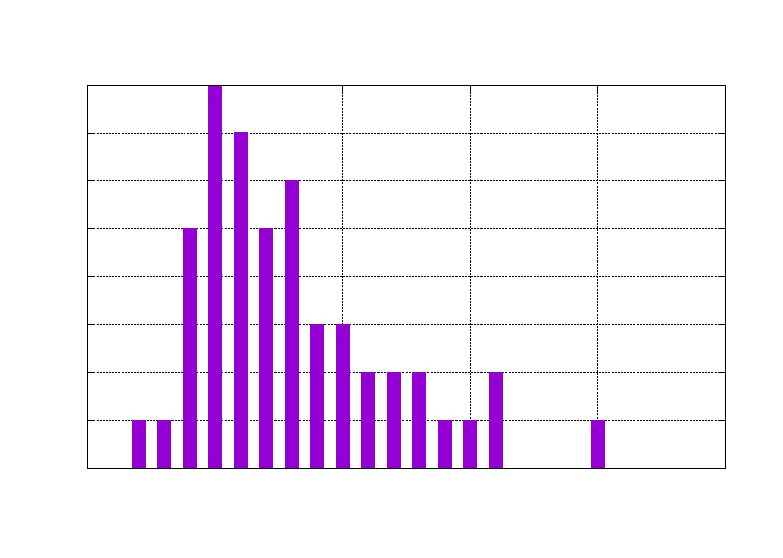
\includegraphics{plots/plot_3-2_h4s0_indegrees}}%
    \gplfronttext
  \end{picture}%
\endgroup

    \caption{Task 3.2: In-degrees (50 Peers, H=4, S=0)}
    \label{fig:3-2_h4s0_indegrees}
\end{figure}

\begin{figure}
    % GNUPLOT: LaTeX picture with Postscript
\begingroup
  \makeatletter
  \providecommand\color[2][]{%
    \GenericError{(gnuplot) \space\space\space\@spaces}{%
      Package color not loaded in conjunction with
      terminal option `colourtext'%
    }{See the gnuplot documentation for explanation.%
    }{Either use 'blacktext' in gnuplot or load the package
      color.sty in LaTeX.}%
    \renewcommand\color[2][]{}%
  }%
  \providecommand\includegraphics[2][]{%
    \GenericError{(gnuplot) \space\space\space\@spaces}{%
      Package graphicx or graphics not loaded%
    }{See the gnuplot documentation for explanation.%
    }{The gnuplot epslatex terminal needs graphicx.sty or graphics.sty.}%
    \renewcommand\includegraphics[2][]{}%
  }%
  \providecommand\rotatebox[2]{#2}%
  \@ifundefined{ifGPcolor}{%
    \newif\ifGPcolor
    \GPcolorfalse
  }{}%
  \@ifundefined{ifGPblacktext}{%
    \newif\ifGPblacktext
    \GPblacktexttrue
  }{}%
  % define a \g@addto@macro without @ in the name:
  \let\gplgaddtomacro\g@addto@macro
  % define empty templates for all commands taking text:
  \gdef\gplbacktext{}%
  \gdef\gplfronttext{}%
  \makeatother
  \ifGPblacktext
    % no textcolor at all
    \def\colorrgb#1{}%
    \def\colorgray#1{}%
  \else
    % gray or color?
    \ifGPcolor
      \def\colorrgb#1{\color[rgb]{#1}}%
      \def\colorgray#1{\color[gray]{#1}}%
      \expandafter\def\csname LTw\endcsname{\color{white}}%
      \expandafter\def\csname LTb\endcsname{\color{black}}%
      \expandafter\def\csname LTa\endcsname{\color{black}}%
      \expandafter\def\csname LT0\endcsname{\color[rgb]{1,0,0}}%
      \expandafter\def\csname LT1\endcsname{\color[rgb]{0,1,0}}%
      \expandafter\def\csname LT2\endcsname{\color[rgb]{0,0,1}}%
      \expandafter\def\csname LT3\endcsname{\color[rgb]{1,0,1}}%
      \expandafter\def\csname LT4\endcsname{\color[rgb]{0,1,1}}%
      \expandafter\def\csname LT5\endcsname{\color[rgb]{1,1,0}}%
      \expandafter\def\csname LT6\endcsname{\color[rgb]{0,0,0}}%
      \expandafter\def\csname LT7\endcsname{\color[rgb]{1,0.3,0}}%
      \expandafter\def\csname LT8\endcsname{\color[rgb]{0.5,0.5,0.5}}%
    \else
      % gray
      \def\colorrgb#1{\color{black}}%
      \def\colorgray#1{\color[gray]{#1}}%
      \expandafter\def\csname LTw\endcsname{\color{white}}%
      \expandafter\def\csname LTb\endcsname{\color{black}}%
      \expandafter\def\csname LTa\endcsname{\color{black}}%
      \expandafter\def\csname LT0\endcsname{\color{black}}%
      \expandafter\def\csname LT1\endcsname{\color{black}}%
      \expandafter\def\csname LT2\endcsname{\color{black}}%
      \expandafter\def\csname LT3\endcsname{\color{black}}%
      \expandafter\def\csname LT4\endcsname{\color{black}}%
      \expandafter\def\csname LT5\endcsname{\color{black}}%
      \expandafter\def\csname LT6\endcsname{\color{black}}%
      \expandafter\def\csname LT7\endcsname{\color{black}}%
      \expandafter\def\csname LT8\endcsname{\color{black}}%
    \fi
  \fi
    \setlength{\unitlength}{0.0500bp}%
    \ifx\gptboxheight\undefined%
      \newlength{\gptboxheight}%
      \newlength{\gptboxwidth}%
      \newsavebox{\gptboxtext}%
    \fi%
    \setlength{\fboxrule}{0.5pt}%
    \setlength{\fboxsep}{1pt}%
\begin{picture}(7200.00,5040.00)%
    \gplgaddtomacro\gplbacktext{%
      \csname LTb\endcsname%
      \put(946,704){\makebox(0,0)[r]{\strut{}$0$}}%
      \csname LTb\endcsname%
      \put(946,1163){\makebox(0,0)[r]{\strut{}$0.05$}}%
      \csname LTb\endcsname%
      \put(946,1623){\makebox(0,0)[r]{\strut{}$0.1$}}%
      \csname LTb\endcsname%
      \put(946,2082){\makebox(0,0)[r]{\strut{}$0.15$}}%
      \csname LTb\endcsname%
      \put(946,2542){\makebox(0,0)[r]{\strut{}$0.2$}}%
      \csname LTb\endcsname%
      \put(946,3001){\makebox(0,0)[r]{\strut{}$0.25$}}%
      \csname LTb\endcsname%
      \put(946,3460){\makebox(0,0)[r]{\strut{}$0.3$}}%
      \csname LTb\endcsname%
      \put(946,3920){\makebox(0,0)[r]{\strut{}$0.35$}}%
      \csname LTb\endcsname%
      \put(946,4379){\makebox(0,0)[r]{\strut{}$0.4$}}%
      \csname LTb\endcsname%
      \put(1078,484){\makebox(0,0){\strut{}$0$}}%
      \csname LTb\endcsname%
      \put(2223,484){\makebox(0,0){\strut{}$10$}}%
      \csname LTb\endcsname%
      \put(3368,484){\makebox(0,0){\strut{}$20$}}%
      \csname LTb\endcsname%
      \put(4513,484){\makebox(0,0){\strut{}$30$}}%
      \csname LTb\endcsname%
      \put(5658,484){\makebox(0,0){\strut{}$40$}}%
      \csname LTb\endcsname%
      \put(6803,484){\makebox(0,0){\strut{}$50$}}%
    }%
    \gplgaddtomacro\gplfronttext{%
      \csname LTb\endcsname%
      \put(176,2541){\rotatebox{-270}{\makebox(0,0){\strut{}Clustering}}}%
      \put(3940,154){\makebox(0,0){\strut{}Peers (cumulated)}}%
      \put(3940,4709){\makebox(0,0){\strut{}Clustering Distribution for H=0 S=4}}%
    }%
    \gplbacktext
    \put(0,0){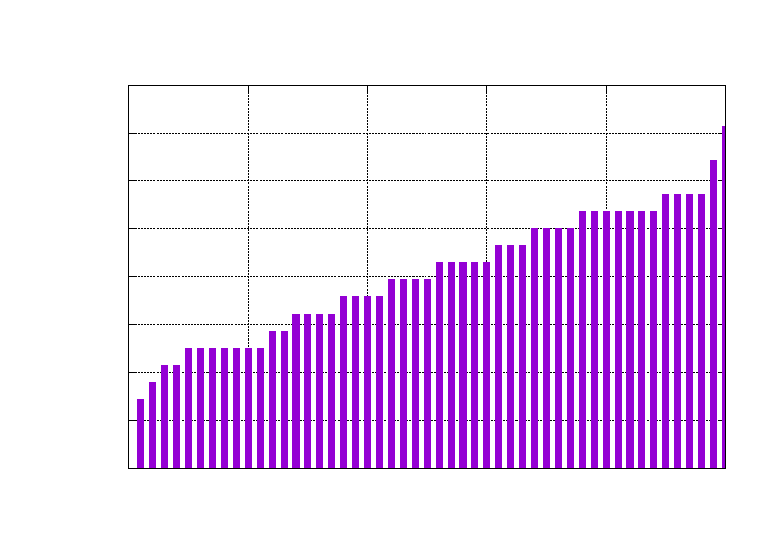
\includegraphics{plots/plot_3-2_h0s4_clustering}}%
    \gplfronttext
  \end{picture}%
\endgroup

    \caption{Task 3.2: Clustering (50 Peers, H=0, S=0)}
    \label{fig:3-2_h0s4_clustering}
\end{figure}

\begin{figure}
    % GNUPLOT: LaTeX picture with Postscript
\begingroup
  \makeatletter
  \providecommand\color[2][]{%
    \GenericError{(gnuplot) \space\space\space\@spaces}{%
      Package color not loaded in conjunction with
      terminal option `colourtext'%
    }{See the gnuplot documentation for explanation.%
    }{Either use 'blacktext' in gnuplot or load the package
      color.sty in LaTeX.}%
    \renewcommand\color[2][]{}%
  }%
  \providecommand\includegraphics[2][]{%
    \GenericError{(gnuplot) \space\space\space\@spaces}{%
      Package graphicx or graphics not loaded%
    }{See the gnuplot documentation for explanation.%
    }{The gnuplot epslatex terminal needs graphicx.sty or graphics.sty.}%
    \renewcommand\includegraphics[2][]{}%
  }%
  \providecommand\rotatebox[2]{#2}%
  \@ifundefined{ifGPcolor}{%
    \newif\ifGPcolor
    \GPcolorfalse
  }{}%
  \@ifundefined{ifGPblacktext}{%
    \newif\ifGPblacktext
    \GPblacktexttrue
  }{}%
  % define a \g@addto@macro without @ in the name:
  \let\gplgaddtomacro\g@addto@macro
  % define empty templates for all commands taking text:
  \gdef\gplbacktext{}%
  \gdef\gplfronttext{}%
  \makeatother
  \ifGPblacktext
    % no textcolor at all
    \def\colorrgb#1{}%
    \def\colorgray#1{}%
  \else
    % gray or color?
    \ifGPcolor
      \def\colorrgb#1{\color[rgb]{#1}}%
      \def\colorgray#1{\color[gray]{#1}}%
      \expandafter\def\csname LTw\endcsname{\color{white}}%
      \expandafter\def\csname LTb\endcsname{\color{black}}%
      \expandafter\def\csname LTa\endcsname{\color{black}}%
      \expandafter\def\csname LT0\endcsname{\color[rgb]{1,0,0}}%
      \expandafter\def\csname LT1\endcsname{\color[rgb]{0,1,0}}%
      \expandafter\def\csname LT2\endcsname{\color[rgb]{0,0,1}}%
      \expandafter\def\csname LT3\endcsname{\color[rgb]{1,0,1}}%
      \expandafter\def\csname LT4\endcsname{\color[rgb]{0,1,1}}%
      \expandafter\def\csname LT5\endcsname{\color[rgb]{1,1,0}}%
      \expandafter\def\csname LT6\endcsname{\color[rgb]{0,0,0}}%
      \expandafter\def\csname LT7\endcsname{\color[rgb]{1,0.3,0}}%
      \expandafter\def\csname LT8\endcsname{\color[rgb]{0.5,0.5,0.5}}%
    \else
      % gray
      \def\colorrgb#1{\color{black}}%
      \def\colorgray#1{\color[gray]{#1}}%
      \expandafter\def\csname LTw\endcsname{\color{white}}%
      \expandafter\def\csname LTb\endcsname{\color{black}}%
      \expandafter\def\csname LTa\endcsname{\color{black}}%
      \expandafter\def\csname LT0\endcsname{\color{black}}%
      \expandafter\def\csname LT1\endcsname{\color{black}}%
      \expandafter\def\csname LT2\endcsname{\color{black}}%
      \expandafter\def\csname LT3\endcsname{\color{black}}%
      \expandafter\def\csname LT4\endcsname{\color{black}}%
      \expandafter\def\csname LT5\endcsname{\color{black}}%
      \expandafter\def\csname LT6\endcsname{\color{black}}%
      \expandafter\def\csname LT7\endcsname{\color{black}}%
      \expandafter\def\csname LT8\endcsname{\color{black}}%
    \fi
  \fi
    \setlength{\unitlength}{0.0500bp}%
    \ifx\gptboxheight\undefined%
      \newlength{\gptboxheight}%
      \newlength{\gptboxwidth}%
      \newsavebox{\gptboxtext}%
    \fi%
    \setlength{\fboxrule}{0.5pt}%
    \setlength{\fboxsep}{1pt}%
\begin{picture}(7200.00,5040.00)%
    \gplgaddtomacro\gplbacktext{%
      \csname LTb\endcsname%
      \put(682,704){\makebox(0,0)[r]{\strut{}$0$}}%
      \csname LTb\endcsname%
      \put(682,1317){\makebox(0,0)[r]{\strut{}$2$}}%
      \csname LTb\endcsname%
      \put(682,1929){\makebox(0,0)[r]{\strut{}$4$}}%
      \csname LTb\endcsname%
      \put(682,2542){\makebox(0,0)[r]{\strut{}$6$}}%
      \csname LTb\endcsname%
      \put(682,3154){\makebox(0,0)[r]{\strut{}$8$}}%
      \csname LTb\endcsname%
      \put(682,3767){\makebox(0,0)[r]{\strut{}$10$}}%
      \csname LTb\endcsname%
      \put(682,4379){\makebox(0,0)[r]{\strut{}$12$}}%
      \csname LTb\endcsname%
      \put(814,484){\makebox(0,0){\strut{}$0$}}%
      \csname LTb\endcsname%
      \put(1670,484){\makebox(0,0){\strut{}$2$}}%
      \csname LTb\endcsname%
      \put(2525,484){\makebox(0,0){\strut{}$4$}}%
      \csname LTb\endcsname%
      \put(3381,484){\makebox(0,0){\strut{}$6$}}%
      \csname LTb\endcsname%
      \put(4236,484){\makebox(0,0){\strut{}$8$}}%
      \csname LTb\endcsname%
      \put(5092,484){\makebox(0,0){\strut{}$10$}}%
      \csname LTb\endcsname%
      \put(5947,484){\makebox(0,0){\strut{}$12$}}%
      \csname LTb\endcsname%
      \put(6803,484){\makebox(0,0){\strut{}$14$}}%
    }%
    \gplgaddtomacro\gplfronttext{%
      \csname LTb\endcsname%
      \put(176,2541){\rotatebox{-270}{\makebox(0,0){\strut{}Number of Nodes}}}%
      \put(3808,154){\makebox(0,0){\strut{}In-Degree}}%
      \put(3808,4709){\makebox(0,0){\strut{}In-degree Distribution for H=0 S=4}}%
    }%
    \gplbacktext
    \put(0,0){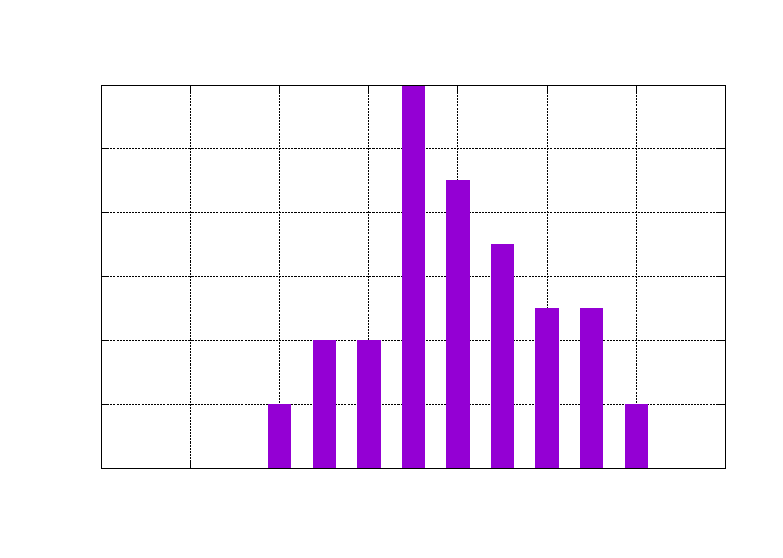
\includegraphics{plots/plot_3-2_h0s4_indegrees}}%
    \gplfronttext
  \end{picture}%
\endgroup

    \caption{Task 3.2: In-degrees (50 Peers, H=0, S=4)}
    \label{fig:3-2_h0s4_indegrees}
\end{figure}

The In-degree and clustering graphs can be seen in figures \ref{fig:3-2_h1s1_indegrees} and \ref{fig:3-2_h1s1_clustering}, respectively.

Varying the H and S parameters as recommended gives the results listed in graphs \ref{fig:3-2_h0s0_clustering} to \ref{fig:3-2_h0s4_indegrees}.

\section{Task 4.1}

This switch is implemented in gossip.lua. if the do\textunderscore peer \textunderscore sampling flag is set, the methods for returning peers for the dissemination protocols take their peers from the local view. Otherwise, they take them from the total list of available nodes.

\section{Task 4.2}

\begin{lstlisting}
---START CONFIG SECTION---
do_rumor_mongering = true
do_anti_entropy = true
do_peer_sampling = true
gossip_interval = 2
peer_sampling_interval = 5
initial_hops_to_live = 4
distribution_count = 3
peer_sampling_view_size = 8
peer_sampling_exchange_rate = 3
peer_sampling_healer_parameter = 0
peer_sampling_shuffler_parameter = 0
peer_selection_policy = "rand"
max_cycles = 10
start_gossipping_after_cycles = 5
---END CONFIG SECTION---

\end{lstlisting}

\begin{figure}
    % GNUPLOT: LaTeX picture with Postscript
\begingroup
  \makeatletter
  \providecommand\color[2][]{%
    \GenericError{(gnuplot) \space\space\space\@spaces}{%
      Package color not loaded in conjunction with
      terminal option `colourtext'%
    }{See the gnuplot documentation for explanation.%
    }{Either use 'blacktext' in gnuplot or load the package
      color.sty in LaTeX.}%
    \renewcommand\color[2][]{}%
  }%
  \providecommand\includegraphics[2][]{%
    \GenericError{(gnuplot) \space\space\space\@spaces}{%
      Package graphicx or graphics not loaded%
    }{See the gnuplot documentation for explanation.%
    }{The gnuplot epslatex terminal needs graphicx.sty or graphics.sty.}%
    \renewcommand\includegraphics[2][]{}%
  }%
  \providecommand\rotatebox[2]{#2}%
  \@ifundefined{ifGPcolor}{%
    \newif\ifGPcolor
    \GPcolorfalse
  }{}%
  \@ifundefined{ifGPblacktext}{%
    \newif\ifGPblacktext
    \GPblacktexttrue
  }{}%
  % define a \g@addto@macro without @ in the name:
  \let\gplgaddtomacro\g@addto@macro
  % define empty templates for all commands taking text:
  \gdef\gplbacktext{}%
  \gdef\gplfronttext{}%
  \makeatother
  \ifGPblacktext
    % no textcolor at all
    \def\colorrgb#1{}%
    \def\colorgray#1{}%
  \else
    % gray or color?
    \ifGPcolor
      \def\colorrgb#1{\color[rgb]{#1}}%
      \def\colorgray#1{\color[gray]{#1}}%
      \expandafter\def\csname LTw\endcsname{\color{white}}%
      \expandafter\def\csname LTb\endcsname{\color{black}}%
      \expandafter\def\csname LTa\endcsname{\color{black}}%
      \expandafter\def\csname LT0\endcsname{\color[rgb]{1,0,0}}%
      \expandafter\def\csname LT1\endcsname{\color[rgb]{0,1,0}}%
      \expandafter\def\csname LT2\endcsname{\color[rgb]{0,0,1}}%
      \expandafter\def\csname LT3\endcsname{\color[rgb]{1,0,1}}%
      \expandafter\def\csname LT4\endcsname{\color[rgb]{0,1,1}}%
      \expandafter\def\csname LT5\endcsname{\color[rgb]{1,1,0}}%
      \expandafter\def\csname LT6\endcsname{\color[rgb]{0,0,0}}%
      \expandafter\def\csname LT7\endcsname{\color[rgb]{1,0.3,0}}%
      \expandafter\def\csname LT8\endcsname{\color[rgb]{0.5,0.5,0.5}}%
    \else
      % gray
      \def\colorrgb#1{\color{black}}%
      \def\colorgray#1{\color[gray]{#1}}%
      \expandafter\def\csname LTw\endcsname{\color{white}}%
      \expandafter\def\csname LTb\endcsname{\color{black}}%
      \expandafter\def\csname LTa\endcsname{\color{black}}%
      \expandafter\def\csname LT0\endcsname{\color{black}}%
      \expandafter\def\csname LT1\endcsname{\color{black}}%
      \expandafter\def\csname LT2\endcsname{\color{black}}%
      \expandafter\def\csname LT3\endcsname{\color{black}}%
      \expandafter\def\csname LT4\endcsname{\color{black}}%
      \expandafter\def\csname LT5\endcsname{\color{black}}%
      \expandafter\def\csname LT6\endcsname{\color{black}}%
      \expandafter\def\csname LT7\endcsname{\color{black}}%
      \expandafter\def\csname LT8\endcsname{\color{black}}%
    \fi
  \fi
    \setlength{\unitlength}{0.0500bp}%
    \ifx\gptboxheight\undefined%
      \newlength{\gptboxheight}%
      \newlength{\gptboxwidth}%
      \newsavebox{\gptboxtext}%
    \fi%
    \setlength{\fboxrule}{0.5pt}%
    \setlength{\fboxsep}{1pt}%
\begin{picture}(7200.00,5040.00)%
    \gplgaddtomacro\gplbacktext{%
      \csname LTb\endcsname%
      \put(682,704){\makebox(0,0)[r]{\strut{}$0$}}%
      \csname LTb\endcsname%
      \put(682,1439){\makebox(0,0)[r]{\strut{}$10$}}%
      \csname LTb\endcsname%
      \put(682,2174){\makebox(0,0)[r]{\strut{}$20$}}%
      \csname LTb\endcsname%
      \put(682,2909){\makebox(0,0)[r]{\strut{}$30$}}%
      \csname LTb\endcsname%
      \put(682,3644){\makebox(0,0)[r]{\strut{}$40$}}%
      \csname LTb\endcsname%
      \put(682,4379){\makebox(0,0)[r]{\strut{}$50$}}%
      \csname LTb\endcsname%
      \put(814,484){\makebox(0,0){\strut{}$2$}}%
      \csname LTb\endcsname%
      \put(2012,484){\makebox(0,0){\strut{}$4$}}%
      \csname LTb\endcsname%
      \put(3210,484){\makebox(0,0){\strut{}$6$}}%
      \csname LTb\endcsname%
      \put(4407,484){\makebox(0,0){\strut{}$8$}}%
      \csname LTb\endcsname%
      \put(5605,484){\makebox(0,0){\strut{}$10$}}%
      \csname LTb\endcsname%
      \put(6803,484){\makebox(0,0){\strut{}$12$}}%
    }%
    \gplgaddtomacro\gplfronttext{%
      \csname LTb\endcsname%
      \put(176,2541){\rotatebox{-270}{\makebox(0,0){\strut{}Peers Infected}}}%
      \put(3808,154){\makebox(0,0){\strut{}Cycles}}%
      \put(3808,4709){\makebox(0,0){\strut{}Dissemination Comparison}}%
      \csname LTb\endcsname%
      \put(5816,2197){\makebox(0,0)[r]{\strut{}H=0 S=0 (19 duplicates)}}%
      \csname LTb\endcsname%
      \put(5816,1977){\makebox(0,0)[r]{\strut{}H=1 S=1 (19 duplicates)}}%
      \csname LTb\endcsname%
      \put(5816,1757){\makebox(0,0)[r]{\strut{}H=1 S=4 (22 duplicates)}}%
      \csname LTb\endcsname%
      \put(5816,1537){\makebox(0,0)[r]{\strut{}H=4 S=0 (19 duplicates)}}%
      \csname LTb\endcsname%
      \put(5816,1317){\makebox(0,0)[r]{\strut{}H=4 S=1 (19 duplicates)}}%
      \csname LTb\endcsname%
      \put(5816,1097){\makebox(0,0)[r]{\strut{}H=0 S=4 (22 duplicates)}}%
      \csname LTb\endcsname%
      \put(5816,877){\makebox(0,0)[r]{\strut{}No Peer Sampling (87 duplicates)}}%
    }%
    \gplbacktext
    \put(0,0){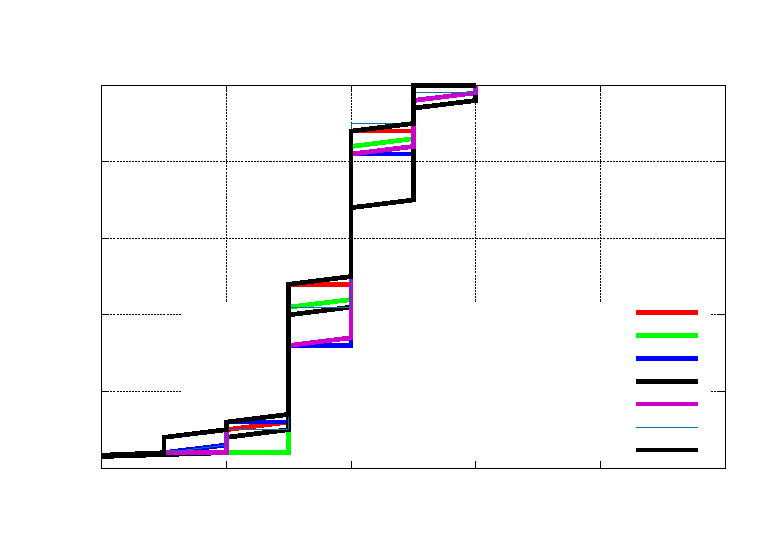
\includegraphics{plots/plot_4-2}}%
    \gplfronttext
  \end{picture}%
\endgroup

    \caption{Task 4.2: Dissemination Comparison with Peer Sampling}
    \label{fig:4-2}
\end{figure}

\begin{figure}
    % GNUPLOT: LaTeX picture with Postscript
\begingroup
  \makeatletter
  \providecommand\color[2][]{%
    \GenericError{(gnuplot) \space\space\space\@spaces}{%
      Package color not loaded in conjunction with
      terminal option `colourtext'%
    }{See the gnuplot documentation for explanation.%
    }{Either use 'blacktext' in gnuplot or load the package
      color.sty in LaTeX.}%
    \renewcommand\color[2][]{}%
  }%
  \providecommand\includegraphics[2][]{%
    \GenericError{(gnuplot) \space\space\space\@spaces}{%
      Package graphicx or graphics not loaded%
    }{See the gnuplot documentation for explanation.%
    }{The gnuplot epslatex terminal needs graphicx.sty or graphics.sty.}%
    \renewcommand\includegraphics[2][]{}%
  }%
  \providecommand\rotatebox[2]{#2}%
  \@ifundefined{ifGPcolor}{%
    \newif\ifGPcolor
    \GPcolorfalse
  }{}%
  \@ifundefined{ifGPblacktext}{%
    \newif\ifGPblacktext
    \GPblacktexttrue
  }{}%
  % define a \g@addto@macro without @ in the name:
  \let\gplgaddtomacro\g@addto@macro
  % define empty templates for all commands taking text:
  \gdef\gplbacktext{}%
  \gdef\gplfronttext{}%
  \makeatother
  \ifGPblacktext
    % no textcolor at all
    \def\colorrgb#1{}%
    \def\colorgray#1{}%
  \else
    % gray or color?
    \ifGPcolor
      \def\colorrgb#1{\color[rgb]{#1}}%
      \def\colorgray#1{\color[gray]{#1}}%
      \expandafter\def\csname LTw\endcsname{\color{white}}%
      \expandafter\def\csname LTb\endcsname{\color{black}}%
      \expandafter\def\csname LTa\endcsname{\color{black}}%
      \expandafter\def\csname LT0\endcsname{\color[rgb]{1,0,0}}%
      \expandafter\def\csname LT1\endcsname{\color[rgb]{0,1,0}}%
      \expandafter\def\csname LT2\endcsname{\color[rgb]{0,0,1}}%
      \expandafter\def\csname LT3\endcsname{\color[rgb]{1,0,1}}%
      \expandafter\def\csname LT4\endcsname{\color[rgb]{0,1,1}}%
      \expandafter\def\csname LT5\endcsname{\color[rgb]{1,1,0}}%
      \expandafter\def\csname LT6\endcsname{\color[rgb]{0,0,0}}%
      \expandafter\def\csname LT7\endcsname{\color[rgb]{1,0.3,0}}%
      \expandafter\def\csname LT8\endcsname{\color[rgb]{0.5,0.5,0.5}}%
    \else
      % gray
      \def\colorrgb#1{\color{black}}%
      \def\colorgray#1{\color[gray]{#1}}%
      \expandafter\def\csname LTw\endcsname{\color{white}}%
      \expandafter\def\csname LTb\endcsname{\color{black}}%
      \expandafter\def\csname LTa\endcsname{\color{black}}%
      \expandafter\def\csname LT0\endcsname{\color{black}}%
      \expandafter\def\csname LT1\endcsname{\color{black}}%
      \expandafter\def\csname LT2\endcsname{\color{black}}%
      \expandafter\def\csname LT3\endcsname{\color{black}}%
      \expandafter\def\csname LT4\endcsname{\color{black}}%
      \expandafter\def\csname LT5\endcsname{\color{black}}%
      \expandafter\def\csname LT6\endcsname{\color{black}}%
      \expandafter\def\csname LT7\endcsname{\color{black}}%
      \expandafter\def\csname LT8\endcsname{\color{black}}%
    \fi
  \fi
    \setlength{\unitlength}{0.0500bp}%
    \ifx\gptboxheight\undefined%
      \newlength{\gptboxheight}%
      \newlength{\gptboxwidth}%
      \newsavebox{\gptboxtext}%
    \fi%
    \setlength{\fboxrule}{0.5pt}%
    \setlength{\fboxsep}{1pt}%
\begin{picture}(7200.00,5040.00)%
    \gplgaddtomacro\gplbacktext{%
      \csname LTb\endcsname%
      \put(682,704){\makebox(0,0)[r]{\strut{}$0$}}%
      \csname LTb\endcsname%
      \put(682,1439){\makebox(0,0)[r]{\strut{}$10$}}%
      \csname LTb\endcsname%
      \put(682,2174){\makebox(0,0)[r]{\strut{}$20$}}%
      \csname LTb\endcsname%
      \put(682,2909){\makebox(0,0)[r]{\strut{}$30$}}%
      \csname LTb\endcsname%
      \put(682,3644){\makebox(0,0)[r]{\strut{}$40$}}%
      \csname LTb\endcsname%
      \put(682,4379){\makebox(0,0)[r]{\strut{}$50$}}%
      \csname LTb\endcsname%
      \put(814,484){\makebox(0,0){\strut{}$8$}}%
      \csname LTb\endcsname%
      \put(1413,484){\makebox(0,0){\strut{}$9$}}%
      \csname LTb\endcsname%
      \put(2012,484){\makebox(0,0){\strut{}$10$}}%
      \csname LTb\endcsname%
      \put(2611,484){\makebox(0,0){\strut{}$11$}}%
      \csname LTb\endcsname%
      \put(3210,484){\makebox(0,0){\strut{}$12$}}%
      \csname LTb\endcsname%
      \put(3809,484){\makebox(0,0){\strut{}$13$}}%
      \csname LTb\endcsname%
      \put(4407,484){\makebox(0,0){\strut{}$14$}}%
      \csname LTb\endcsname%
      \put(5006,484){\makebox(0,0){\strut{}$15$}}%
      \csname LTb\endcsname%
      \put(5605,484){\makebox(0,0){\strut{}$16$}}%
      \csname LTb\endcsname%
      \put(6204,484){\makebox(0,0){\strut{}$17$}}%
      \csname LTb\endcsname%
      \put(6803,484){\makebox(0,0){\strut{}$18$}}%
    }%
    \gplgaddtomacro\gplfronttext{%
      \csname LTb\endcsname%
      \put(176,2541){\rotatebox{-270}{\makebox(0,0){\strut{}Peers Infected}}}%
      \put(3808,154){\makebox(0,0){\strut{}Seconds}}%
      \put(3808,4709){\makebox(0,0){\strut{}Dissemination Comparison}}%
      \csname LTb\endcsname%
      \put(5816,2197){\makebox(0,0)[r]{\strut{}H=0 S=0}}%
      \csname LTb\endcsname%
      \put(5816,1977){\makebox(0,0)[r]{\strut{}H=1 S=1}}%
      \csname LTb\endcsname%
      \put(5816,1757){\makebox(0,0)[r]{\strut{}H=1 S=4}}%
      \csname LTb\endcsname%
      \put(5816,1537){\makebox(0,0)[r]{\strut{}H=4 S=0}}%
      \csname LTb\endcsname%
      \put(5816,1317){\makebox(0,0)[r]{\strut{}H=4 S=1}}%
      \csname LTb\endcsname%
      \put(5816,1097){\makebox(0,0)[r]{\strut{}H=0 S=4}}%
      \csname LTb\endcsname%
      \put(5816,877){\makebox(0,0)[r]{\strut{}No PSS}}%
    }%
    \gplbacktext
    \put(0,0){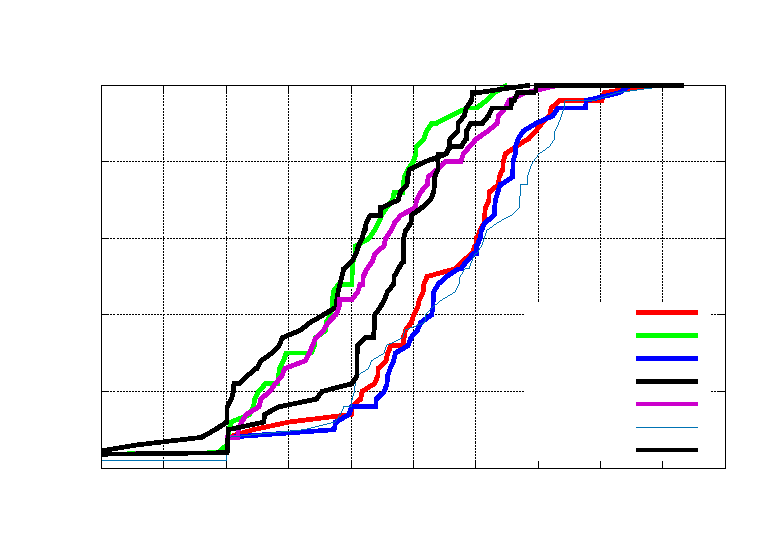
\includegraphics{plots/plot_4-2_seconds}}%
    \gplfronttext
  \end{picture}%
\endgroup

    \caption{Task 4.2: Dissemination Comparison with Peer Sampling}
    \label{fig:4-2_seconds}
\end{figure}

Finally, I compared various values of healer and shuffler parameters and plottet the results. I used the above configuration, with changed values in the peer\textunderscore sampling\textunderscore healer\textunderscore parameter and peer\textunderscore sampling\textunderscore shuffler\textunderscore parameter. The results can be found in figure \ref{fig:4-2}. In this figure you can also see the duplicate rates.
For this particular graph, I wanted to see the results in seconds too, so I added an additional plot with seconds on the x axis in figure \ref{fig:4-2_seconds}.

\end{document}
